\documentclass[12pt]{article}

%%%%%%%%%%%%%%%%%%%%%%%%%%%%%%%%%%%%%%%%%%%%%%%%%%%%%%%%%%%%%%%%%%%%%%%%%%%%%%%%
%                           Package preset for homework
%%%%%%%%%%%%%%%%%%%%%%%%%%%%%%%%%%%%%%%%%%%%%%%%%%%%%%%%%%%%%%%%%%%%%%%%%%%%%%%%
% Miscellaneous
\usepackage[margin=1in]{geometry}
\usepackage[utf8]{inputenc}
\usepackage{indentfirst}
\usepackage{blindtext}
\usepackage{graphicx}
\usepackage{xr-hyper}
\usepackage{hyperref}
\usepackage{enumitem}
\usepackage{color}
\usepackage{float}
% Math
\usepackage{latexsym}
\usepackage{amsfonts}
\usepackage{amssymb}
\usepackage{amsmath}
\usepackage{commath}
\usepackage{amsthm}
\usepackage{bbold}
\usepackage{bm}
% Physics
\usepackage{physics}
\usepackage{siunitx}
% Code typesetting
\usepackage{listings}
% Citation
\usepackage[authoryear]{natbib}
\usepackage{appendix}
\usepackage[capitalize]{cleveref}
% Title & name
\title{Homework}
\author{Tien Vo}
\date{\today}


%%%%%%%%%%%%%%%%%%%%%%%%%%%%%%%%%%%%%%%%%%%%%%%%%%%%%%%%%%%%%%%%%%%%%%%%%%%%%%%%
%                   User-defined commands and environments
%%%%%%%%%%%%%%%%%%%%%%%%%%%%%%%%%%%%%%%%%%%%%%%%%%%%%%%%%%%%%%%%%%%%%%%%%%%%%%%%
%%% Misc
\sisetup{load-configurations=abbreviations}
\newcommand{\due}[1]{\date{Due: #1}}
\newcommand{\hint}{\textit{Hint}}
\let\oldt\t
\renewcommand{\t}[1]{\text{#1}}

%%% Bold sets & abbrv
\newcommand{\N}{\mathbb{N}}
\newcommand{\Z}{\mathbb{Z}}
\newcommand{\R}{\mathbb{R}}
\newcommand{\Q}{\mathbb{Q}}
\let\oldP\P
\renewcommand{\P}{\mathbb{P}}
\newcommand{\LL}{\mathcal{L}}
\newcommand{\FF}{\mathcal{F}}
\newcommand{\HH}{\mathcal{H}}
\newcommand{\NN}{\mathcal{N}}
\newcommand{\ZZ}{\mathcal{Z}}
\newcommand{\RN}[1]{\textup{\uppercase\expandafter{\romannumeral#1}}}
\newcommand{\ua}{\uparrow}
\newcommand{\da}{\downarrow}

%%% Unit vectors
\newcommand{\xhat}{\vb{\hat{x}}}
\newcommand{\yhat}{\vb{\hat{y}}}
\newcommand{\zhat}{\vb{\hat{z}}}
\newcommand{\nhat}{\vb{\hat{n}}}
\newcommand{\rhat}{\vb{\hat{r}}}
\newcommand{\phihat}{\bm{\hat{\phi}}}
\newcommand{\thetahat}{\bm{\hat{\theta}}}

%%% Other math stuff
\providecommand{\units}[1]{\,\ensuremath{\mathrm{#1}}\xspace}
% Set new style for problem
\newtheoremstyle{problemstyle}  % <name>
        {10pt}                   % <space above>
        {10pt}                   % <space below>
        {\normalfont}           % <body font>
        {}                      % <indent amount}
        {\bfseries\itshape}     % <theorem head font>
        {\normalfont\bfseries:} % <punctuation after theorem head>
        {.5em}                  % <space after theorem head>
        {}                      % <theorem head spec (can be left empty, 
                                % meaning `normal')>

% Set problem environment
\theoremstyle{problemstyle}
\newtheorem{problemenv}{Problem}[section]
\newenvironment{problem}[1]{%
  \renewcommand\theproblemenv{#1}%
  \problemenv
}{\endproblemenv}
% Set lemma environment
\newenvironment{lemma}[2][Lemma]{\begin{trivlist}
\item[\hskip \labelsep {\bfseries #1}\hskip \labelsep {\bfseries #2.}]}{\end{trivlist}}
% Set solution environment
\newenvironment{solution}{
    \begin{proof}[Solution]$ $\par\nobreak\ignorespaces
}{\end{proof}}
\numberwithin{equation}{problemenv}

%%% Page format
\setlength{\parindent}{0.5cm}
\setlength{\oddsidemargin}{0in}
\setlength{\textwidth}{6.5in}
\setlength{\textheight}{8.8in}
\setlength{\topmargin}{0in}
\setlength{\headheight}{18pt}

%%% Code environments
\definecolor{dkgreen}{rgb}{0,0.6,0}
\definecolor{gray}{rgb}{0.5,0.5,0.5}
\definecolor{mauve}{rgb}{0.58,0,0.82}
\lstset{frame=tb,
  language=Python,
  aboveskip=3mm,
  belowskip=3mm,
  showstringspaces=false,
  columns=flexible,
  basicstyle={\small\ttfamily},
  numbers=none,
  numberstyle=\tiny\color{gray},
  keywordstyle=\color{blue},
  commentstyle=\color{dkgreen},
  stringstyle=\color{mauve},
  breaklines=true,
  breakatwhitespace=true,
  tabsize=4
}
\lstset{
  language=Mathematica,
  numbers=left,
  numberstyle=\tiny\color{gray},
  numbersep=5pt,
  breaklines=true,
  captionpos={t},
  frame={lines},
  rulecolor=\color{black},
  framerule=0.5pt,
  columns=flexible,
  tabsize=2
}

\usepackage{enumitem}

\title{Homework 5: Phys 7230 (Spring 2022)}
\due{March 30, 2022}

\begin{document}
\maketitle
%%%%%%%%%%%%%%%%%%%%%%%%%%%%%%%%%%%%%%%%%%%%%%%%%%%%%%%%%%%%%%%%%%%%%%%%%%%%%%%
\begin{problem}{1}[Quantum many-body statistics]
Consider a system with 3 single particle nondegenerate energy levels
$\alpha=(a,b,c)$ equally spaced with values
$\epsilon_a=0,\epsilon_b=\epsilon,\epsilon_c=2\epsilon$, and occupied by 2
particles.

(a) Write down the \textit{ground} states for bosons and fermions in three
forms:

\qquad(i) Many-body wavefunction $\psi_{\alpha_1,\alpha_2}(x_1,x_2)$, in terms
of \textit{normalized} single particle wavefunctions
$\psi_\alpha(x)(\alpha=(a,b,c))$, appropriately (anti-)symmetrized using
determinant and permanent method. Make sure that there is a correct overall
normalization.

\qquad(ii) A many-body ket in the occupation basis $\qty{n_\alpha}$
representation, written as, $\ket{n_a,n_b,n_c}=\ket{n_a}\ket{n_b}\ket{n_c}$.

\qquad(iii) Drawing equally spaced energy levels
$\epsilon_a,\epsilon_b,\epsilon_c$ as horizontal lines with ``balls''
representing particles sitting on the levels.
\begin{solution}
(i) For fermions, the ground state has energy $\epsilon$ since they cannot
both occupy $a$. Thus, the wave function is
\begin{equation}
    \psi_{a,b}^F(x_1,x_2)
    =\frac1{\sqrt2}\det\mqty[\psi_a(x_1)&\psi_a(x_2)\\\psi_b(x_1)&\psi_b(x_2)]
    =\frac1{\sqrt2}\qty(\psi_a(x_1)\psi_b(x_2)-\psi_a(x_2)\psi_b(x_1)).
\end{equation}
For bosons, they can both occupy $a$. Thus, the ground state wave function is
\begin{equation}
    \psi_{a,a}^B(x_1,x_2)
    =\frac1{2}\t{Perm}\mqty[\psi_a(x_1)&\psi_a(x_2)\\\psi_a(x_1)&\psi_a(x_2)]
=\psi_a(x_1)\psi_a(x_2).
\end{equation}

(ii) $\ket{\psi_{a,b}^F}=\ket{1,1,0}$ and $\ket{\psi_{a,a}^B}=\ket{2,0,0}$.
\end{solution}

(b) Repeat above many-body state description for the 1st \textit{excited}
many-body states for bosons and fermions.
\begin{solution}
(i) The first excited state for fermions has total energy $2\epsilon$
\begin{equation}
    \psi_{a,c}^F(x_1,x_2)=\frac1{\sqrt2}\qty(\psi_a(x_1)\psi_c(x_2)-\psi_a(x_2)\psi_c(x_1)),
\end{equation}
where we have simply exchanged $b\to c$ from the previous result. For bosons,
one particle occupies $a$ and the other is excited to $b$,
\begin{equation}
    \psi_{a,b}^B(x_1,x_2)=\frac1{\sqrt2}\t{Perm}\mqty[\psi_a(x_1)&\psi_a(x_2)\\\psi_b(x_1)&\psi_b(x_2)]=\frac1{\sqrt2}\qty(\psi_a(x_1)\psi_b(x_2)+\psi_a(x_2)\psi_b(x_1)).
\end{equation}

(ii) $\ket{\psi_{a,c}^F}=\ket{1,0,1}$ and $\ket{\psi_{a,b}^B}=\ket{1,1,0}$.
\end{solution}

(c) Using $\ket{n_a,n_b,n_c}$ labeling list (i) \textit{all} the many-body
eigenstates for this system of 2 particles for bosons and for fermions, (ii)
corresponding many-body energies $E_\qty{n_\alpha}=E_{n_a,n_b,n_c}$, and (iii)
the 2-particle partition function $Z$, explicitly writing out the sum of all
finite number of terms. Do this for both bosons and fermions.
\begin{solution}
(i) 
\begin{itemize}
    \item Fermions:  $\ket{1,1,0},\ket{1,0,1},\ket{0,1,1}$
    \item Bosons: $\ket{2,0,0},\ket{1,1,0},\ket{0,2,0},\ket{1,0,1},\ket{0,1,1},\ket{0,0,2}$
\end{itemize}

(ii)
\begin{itemize}
    \item Fermions: $E_{1,1,0}=\epsilon$, $E_{1,0,1}=2\epsilon$,
        $E_{0,1,1}=3\epsilon$ 
    \item Bosons: $E_{2,0,0}=0$, $E_{1,1,0}=\epsilon$,
        $E_{0,2,0}=E_{1,0,1}=2\epsilon$, $E_{0,1,1}=3\epsilon$,
        $E_{0,0,2}=4\epsilon$
\end{itemize}

(iii) For fermions, there is no degeneracy, so
\begin{equation}
    Z^F = \sum_{\qty{q}}e^{-\beta E_q}
    =e^{-\beta\epsilon}+e^{-2\beta\epsilon}+e^{-3\beta\epsilon}.
\end{equation}
For bosons,
\begin{equation}
    Z^B=1+e^{-\beta\epsilon}+2e^{-2\beta\epsilon}
    +e^{-3\beta\epsilon}+e^{-4\beta\epsilon}.
\end{equation}
\end{solution}

(d) Using quantum many-body state labeling $\ket{\alpha_1,\alpha_2}$ where
$\alpha_i$ is the single-particle state ($a,b$, or $c$) occupied by
\textit{distinguishable} particle $i=(1,2)$, write down (i) \textit{all}
many-body states for \textit{distinguishable} particles, (ii) their
corresponding many-body energies $E_{\alpha_1,\alpha_2}$, and (iii) the
2-particle partition function $Z_{N=2}$. Show that this latter sum in $Z_2$ of
many terms can actually be written as a product of 1-particle partition
functions, i.e., $Z_2=Z_1^2$.
\begin{solution}
(i)
$\ket{a,a},\ket{b,b},\ket{c,c},\ket{a,b},\ket{b,a},\ket{a,c},\ket{c,a},\ket{b,c},\ket{c,b}$.
(ii) $E_{a,a}=0,
E_{a,b}=E_{b,a}=\epsilon,E_{a,c}=E_{c,a}=E_{b,b}=2\epsilon,E_{b,c}=E_{c,b}=3\epsilon,E_{c,c}=4\epsilon$.
(iii) It follows from (i) and (ii) that
\begin{equation}
    Z_2=1+2e^{-\beta\epsilon}+3e^{-2\beta\epsilon}+2e^{-3\beta\epsilon}
    +e^{-4\beta\epsilon}.
\end{equation}
For a single particle, the partition function is
\begin{equation}
    Z_1=1+e^{-\beta\epsilon}+e^{-2\beta\epsilon}. 
\end{equation}
Thus, we also have
\begin{align}
    Z_1^2
    &=1+2e^{-\beta\epsilon}+2e^{-2\beta\epsilon}
    +\qty(e^{-\beta\epsilon}+e^{-2\beta\epsilon})^2\notag\\
    &=1+2e^{-\beta\epsilon}+2e^{-2\beta\epsilon}
    +e^{-2\beta\epsilon}+e^{-4\beta\epsilon}+2e^{-3\beta\epsilon}\notag\\
    &=1+2e^{-\beta\epsilon}
    +3e^{-2\beta\epsilon}
    +2e^{-3\beta\epsilon}
    +e^{-4\beta\epsilon}\notag\\
    &=Z_2.
\end{align}
\end{solution}
\end{problem}
\newpage
%%%%%%%%%%%%%%%%%%%%%%%%%%%%%%%%%%%%%%%%%%%%%%%%%%%%%%%%%%%%%%%%%%%%%%%%%%%%%%%    
%%%%%%%%%%%%%%%%%%%%%%%%%%%%%%%%%%%%%%%%%%%%%%%%%%%%%%%%%%%%%%%%%%%%%%%%%%%%%%%
\begin{problem}{2}[Bose gas in a box]
In lectures we introduced noninteracting (ideal) Bose gas in a box (with
periodic boundary conditions) and presented many results, some without
derivations. Here I will ask you to derive some of the details.

(a) Following our derivation of the number equation $\overline{N}$, Eq. 24 from
its definition Eq. 22 in the lecture notes, from the grand canonical partition
function derive the equation of state for the pressure $P$, Eq. 29 and energy
$E$, Eq. 30, Combining these results together with $\overline{N}$, Eq. 24, in
3D, derive the first two virial coefficients for the equation of state (Eq. 31)
at high temperature $T\gg T_\ast$ (nondegenerate gas limit), where $z\ll 1$.
Show that $a_0=1$ and $a_1=-1/2^{5/2}$, as found in Eq. 18 of the notes.

\textit{Hint}: This can be done by a powerful and quite general iterative
perturbation series approach, valid when $z\ll 1$. Suppose you want to solve the
number equation, $n=g(z)=c_1z+c_2z^2+\hdots$, inverting it for $z(n)$ (so you
can later eliminate $z$ from other thermodynamics quantities like $P$). Take the
zeroth order approximation $z\approx z_1$ ignoring $z^2$ and higher order terms,
then the equation above gives $z_1=n/c_1$. Then at next iteraction of the
approximation, you can find $z_2$ by going to 2nd order in $z$ expansion of
$g(z)$, using the unknown $z_2$ inside $c_1z$ but only using the previous 1st
order solution $z_1$ inside $c_2z^2$ and solving for $z_2$, etc. Why do you
think this is justified? This way you will find, $z\approx z_2=b_1n+b_2n^2$,
which is sufficient to compute $P(T,n)$ to 2nd order in $n$ by eliminating $z$
in its Taylor expansion in right hand side of Eq. 31.
\begin{solution}
First, we calculate the free energy (27) in the notes.
\begin{align}
    \FF_B&=k_BT\sum_{\vb{k}}\ln\qty[1-e^{-(\epsilon_{\vb{k}}-\mu)/k_BT}]\notag\\
     &=k_BT\qty(\frac{L}{2\pi})^d
     \int d^dk\ln\qty[1-e^{-(\epsilon-\mu)/k_BT}]\notag\\
     &=k_BT\qty(\frac{L}{2\pi})^dS_d\int_0^\infty dk
     k^{d-1}\ln\qty[1-e^{-(\epsilon-\mu)/k_BT}]\notag\\
     &=\frac{Vk_BT}{2(2\pi)^d}\qty(\frac{2m}{\hbar^2})^{d/2}S_d\int_0^\infty
     d\epsilon
     \epsilon^{d/2-1}\ln\qty[1-e^{-(\epsilon-\mu)/k_BT}]\tag{$\epsilon=\hbar^2k^2/2m$}\\
     &=-\frac{V}{d(2\pi)^d}\qty(\frac{2m}{\hbar^2})^{d/2}S_d\int_0^\infty
     d\epsilon\frac{\epsilon^{d/2}}{e^{(\epsilon-\mu)/k_BT}-1}\notag\\
     &=-\frac2d\frac{Vk_BT}{\Gamma(d/2)}\qty(\frac{mk_BT}{2\pi\hbar^2})^{d/2}\int_0^\infty
     dx\frac{x^{d/2}}{e^xz^{-1}-1}\notag\\
     &=-\frac2d\frac{Vk_BT}{\lambda^d}\frac{\Gamma(d/2+1)}{\Gamma(d/2)}g_{d/2+1}(z)\notag\\
     &=-\frac{Vk_BT}{\lambda^d}g_{d/2+1}(z).
\end{align}
Thus, it follows that
\begin{equation}
    P=-\frac{\FF_B}{V}
    =\frac{k_BT}{\lambda^d}g_{d/2+1}(z).
\end{equation}
Similarly, the energy density is
\begin{align}
    \frac{E}{V}&=-\frac1V\frac{\partial(\ln\ZZ)}{\partial\beta}\notag\\ 
               &=-\frac1V\sum_{\vb{k}}\frac{\partial}{\partial\beta}\ln\qty[1-e^{-(\epsilon-\mu)/k_BT}]^{-1}\notag\\
               &=\frac1{(2\pi)^d}\int
               d^dk\frac{\epsilon-\mu}{e^{(\epsilon-\mu)/k_BT}-1}\notag\\
               &=\frac{1}{(2\pi)^d}\qty(\frac{2m}{\hbar^2})^{d/2}\frac{S_d}{2}\int_0^\infty
               d\epsilon\frac{\epsilon^{d/2}-\mu
               \epsilon^{d/2-1}}{e^{(\epsilon-\mu)/k_BT}-1}\notag\\
               &=\frac{k_BT}{\Gamma(d/2)}\qty(\frac{mk_BT}{2\pi\hbar^2})^{d/2}
               \qty[\int_0^\infty
               dx\frac{x^{d/2}}{e^xz^{-1}-1}-\frac{\mu}{k_BT}\int_0^\infty
               dx\frac{x^{d/2-1}}{e^xz^{-1}-1}]\notag\\
               &=\frac{k_BT}{\lambda^d}\qty[\frac{\Gamma(d/2+1)}{\Gamma(d/2)}g_{d/2+1}(z)-g_{d/2}(z)\ln\qty(g_{d/2}(z))]\notag\\
               &\approx\frac{d}{2}\frac{k_BT}{\lambda^d}g_{d/2+1}(z),
\end{align}
where the second term drops out in the limit that $z\ll 1$. Now, from the
pressure, in 3D, we can write
\begin{equation}
    \frac{PV}{Nk_BT}=\frac{g_{5/2}}{g_{3/2}}
    \approx\frac{z+2^{-5/2}z^2}{z+2^{-3/2}z^2}
    \approx 1-2^{-5/2}z.
\end{equation}
But from (25), $n\lambda^3=g_{3/2}\approx z$, so
\begin{equation}
    \frac{PV}{Nk_BT}\approx1-2^{-5/2}(n\lambda^3). 
\end{equation}
Reading off of this, we know that $a_1=1$ and $a_2=-2^{-5/2}$.
\end{solution}

(b) In lecture I argued that $\mu(T,n)$ is negative for $T\gg T_c$ increases
toward zero (with absolute value $\abs{\mu}$ decreasing to 0) with reduced $T$ 
as it approaches $T_c$ from above. From the defining $N$ equation (23), make the
appropriate approximation (assuming $z\ll1$), neglecting 1 in the denominator
of $n^{BE}(\epsilon_{\vb{k}})$, do the Gaussian integral over $\vb{k}$ and solve
for $\mu(T,n)$ in $d$ dimension.

\textit{Hint}: In Eq. 25, $g_\nu(z)\approx z$ for $z\ll1$, which is another
direct route to your answer above, but use it only as a check.
\begin{solution}
Assuming $\mu\ll 1$, we can write
\begin{align}
    N&\approx\sum_{\vb{k}}e^{-\beta(\epsilon-\mu)}\notag\\
     &=z\qty(\frac{L}{2\pi})^d\int
     d^dk\exp\qty(-\frac12\frac{\beta\hbar^2}{m}k^2)\notag\\
     &=\frac{zV}{(2\pi)^d}\qty[\int
 dk_j\exp\qty(-\frac12\frac{\beta\hbar^2}{m}k_j^2)]^d\notag\\
     &=\frac{zV}{(2\pi)^d}\qty(\frac{2\pi}{\beta\hbar^2/m})^{d/2}\notag\\
     &=zV\qty(\frac{mk_BT}{2\pi\hbar^2})^{d/2}\notag\\
     &=\frac{zV}{\lambda^d}.
\end{align}
Thus, it follows that $z=n\lambda^d$, as expected. Inverting this, we can write
\begin{equation}
    \mu=k_BT\ln\qty(n\lambda^d). 
\end{equation}
\end{solution}

(c) Why do I keep saying that at high $T\gg T_c$ the fugacity $z=e^{\mu(T)/T}\ll
1$ in this limit? Use above derived expression for $\mu(T,n)$ to confirm that
indeed $z(T\gg T_\ast)\ll1$.
\begin{solution}
From above, the fugacity $z\ll 1$ only when $n\lambda^d\ll 1$. This is
equivalent to saying $T\gg T_\ast$. Recall that the degeneracy 
temperature
\begin{equation}
    k_BT_\ast=\frac{\hbar^2n^{2/d}}{2m}, 
\end{equation}
while the temperature defined by the Debye length is
\begin{equation}
    k_BT=\frac{2\pi\hbar^2}{m\lambda^2}. 
\end{equation}
Thus, $k_BT\gg k_BT_\ast$ only when $n\lambda^d\ll (4\pi)^{d/2}\sim\order{1}$.
\end{solution}

(d) Consider the $N$, Eq. 23 again. Based on it I argued that as $T$ is lowered
and $N$ is increased, $\mu$ must increase toward 0, as you verified above. And
in addition, in $d>2$, $\mu(T\to T_c)\to0$, i.e. gets pinned at $\mu=0$. Why do
I insist on this, namely, why can't $\mu$ become positive for $T<T_c$, in its
attempt to satisfy the number equation? Argue for this based on Eqs. 22, 33,
that for noninteracting Bose gas it is unphysical for $\mu$ to become positive.

\textit{Hint}: Above I asked you to argue that the limiting value of $\mu$ is 0.
But on the other hand you know that in physics (other than gravity)
only \textit{relative} energy matter. Based on your previous argument for
$\mu=0$, for $\epsilon_0=\hbar^2k^2/2m$, what do you think the more general
answer for the limiting value of $\mu$ is in the case of the lowest
single-particle energy level $\epsilon_{\alpha=0}=\epsilon_0$ rather than 0?
\begin{solution}
When $\mu$ is positive, the integral is still convergent at a finite value. So
it is not possible to satisfy the number equation for any arbitrary $N$. This
saturation starts at $\mu=0$, so the limiting value for $\mu$ must be zero. Now,
$\mu$ is negative for $T\gg T_c$, so only negative $\mu$ has physical meaning.
If the ground state energy is $\epsilon_0$, then the limiting value of $\mu$ is
$\epsilon_0$ instead.
\end{solution}

(e) From the condition $n\lambda_T(T_c)^d=g_{d/2}(1)$, derive the expression for
$T_c$ as
$k_BT_c=\frac{4\pi}{\zeta(d/2)^{2/d}}\frac{\hbar^2n^{2/d}}{2m}=\frac{4\pi
k_BT_\ast}{\zeta(d/2)^{2/d}}$, valid for $d>2$, and $T_c=6.625T_\ast$ in 3D, as
given in the notes.
\begin{solution}
By definition,
\begin{equation}
    \lambda(T)=\qty(\frac{2\pi\hbar^2}{mk_BT})^{1/2}. 
\end{equation}
Thus,
\begin{equation}
    \zeta(d/2)=n\lambda^d(T_c)=n\qty(\frac{2\pi\hbar^2}{mk_BT_c})^{d/2}. 
\end{equation}
Inverting, we can write
\begin{equation}
    k_BT_c=\frac{2\pi\hbar^2n^{2/d}}{m\zeta^{2/d}(d/2)}=\frac{4\pi}{\zeta^{2/d}(d/2)}\frac{\hbar^2n^{2/d}}{2m}
    =\frac{4\pi}{\zeta^{2/d}(d/2)}k_BT_\ast.
\end{equation}
For $d=3$, we can evaluate the prefactor $4\pi/\zeta^{2/3}(3/2)=6.625$, as given
in the lecture notes.
\end{solution}

(f) As discussed at length in the lecture, for $T<T_c$ the condensation density
$n_0(T)$ becomes nonzero and growing with decreasing $T$ toward the total
density $n$ at $T=0$. Starting with Eq. 35 in the lecture notes,
$n=n_0(T)+\int\frac{d^dk}{(2\pi)^d}\frac1{e^{\beta(\epsilon_{\vb{k}}-\mu)}-1}$,
derive the temperature dependence of $n_0(T)$ for $T<T_c$ given in the notes,
$n_0(T)=n\qty[1-\qty(\frac{T}{T_c})^{d/2}],$

\textit{Hint}: (i) What is the value of $\mu$ for $T<T_c$ that we are exploring
here? (ii) This significantly simplifies ``excitations'' of the number equation
above (Eq. 35 in notes), as one can change variables and scale $T$ out of the
integral. (iii) Note that the value of this last integral at $T_c$ allows us to
eliminate the complicated integral and replace it by a power of $T_c$, thereby
giving the desired simple expression for $n_0(T)$.
\begin{solution}
For $T<T_c$, $\mu\approx 0$. Thus, the integration simplifies to
\begin{align}
    n
    &=n_0+\frac1{(2\pi)^d}\int_0^\infty dk \frac{k^{d-1}}{e^{\beta\epsilon}-1}\notag\\
    &=n_0+\frac1{(2\pi)^d}\qty(\frac{2m}{\hbar^2})^{d/2}\frac{\pi^{d/2}}{\Gamma(d/2)}\int_0^\infty
    d\epsilon\frac{\epsilon^{d/2-1}}{e^{\beta\epsilon}-1}\notag\\
    &=n_0+\frac1{\lambda^d(T)}g_{d/2}(1)\notag\\
    &=n_0+n\qty(\frac{\lambda(T_c)}{\lambda(T)})^d\notag\\
    &=n_0+n\qty(\frac{T}{T_c})^{d/2}.
\end{align}
Thus, as desired,
\begin{equation}
    n_0=n\qty[1-\qty(\frac{T}{T_c})^{d/2}]. 
\end{equation}
\end{solution}

(g) Show that below but close to $T_c$, the condensate density grows as
$n_0(T)\sim T_c-T$.
\begin{solution}
Let $x=T/T_c$, then by a Taylor expansion around $x=1$,
\begin{equation}
    n_0\approx n_0(x=1)+\eval{\frac{\partial n_0}{\partial x}}_{x=1}(x-1)
    =-n\frac{d}{2}1^{d/2-1}(x-1)
    =\frac{nd}{2T_c}(T_c-T)
    \sim T_c-T.
\end{equation}
\end{solution}

(h) Focusing on low temperatures, $T\ll T_c$, derive the power-law excitation
energy $E(T)\sim T^{d/2+1}$ and the corresponding heat capacity $C_v(T)\sim
T^{d/2}$ quoted in the lecture notes.
\begin{solution}
From the result of part (a), at low temperatures, $\mu\approx 0\rightarrow
z\to1$ and
\begin{equation}
    \frac{E}{V}\approx\frac{d}{2}\frac{k_BT}{\lambda_T^d}g_{d/2+1}(1)
    =\frac{d}{2}\zeta(d/2+1)\frac{k_BT}{\lambda_T^d}.
\end{equation}
Since $\lambda_T^d\sim T^{-d/2}$, it then follows that $E\sim T^{d/2+1}$ and
$C_v=\partial E/\partial T\sim T^{d/2}$.
\end{solution}

\end{problem}
\newpage
%%%%%%%%%%%%%%%%%%%%%%%%%%%%%%%%%%%%%%%%%%%%%%%%%%%%%%%%%%%%%%%%%%%%%%%%%%%%%%%

%%%%%%%%%%%%%%%%%%%%%%%%%%%%%%%%%%%%%%%%%%%%%%%%%%%%%%%%%%%%%%%%%%%%%%%%%%%%%%%
\begin{problem}{3}[Bose gas in a harmonic potential]
Consider a gas of noninteracting \textit{bosonic} atoms in a 3-dimensional
\textit{harmonic} potential $V(x,y)=\frac12m\omega_0^2r^2$, as now is routinely
done in JILA and other laboratories around the world (physically the harmonic
potential is typically either optical or magnetic trap). Let us repeat our
in-class and above analysis (for the box with periodic boundary conditions) for
this harmonic potential.

(a) Write down the singe-particle energies for this potential.
\begin{solution}
The single-particle Hamiltonian is
\begin{equation}
    \HH=\qty[\frac{\vb{p}^2}{2m}+\frac12m\omega_0^2\vb{r}^2-\frac32\hbar\omega_0],
\end{equation}
which has the energy eigenvalues
\begin{equation}
    \epsilon_\alpha=\hbar\omega_0(n_x+n_y+n_z), 
\end{equation}
where $\alpha_{\vb{n}}=(n_x,n_y,n_z)$.
\end{solution}

(b) Use the above result and general thermodynamic analysis (e.g., from
lectures) of the Bose gas to write down the $N$ equation as sum over oscillator
single particle quantum states $\alpha_{\vb{n}}=(n_x,n_y,n_z)$ in 3 dimensions.
(For concreteness use the definition of the Hamiltonian such that the ground
state single-particle energy in the trap is at zero, i.e., subtract zero-point
energy).
\begin{solution}
For bosons, the occupation density is
\begin{equation}
    n_\alpha=\frac1{e^{\beta(\epsilon_\alpha-\mu)}-1}. 
\end{equation}
Thus,
\begin{equation}
    N=\sum_\alpha
    n_\alpha=\sum_{\vb{n}}\qty[e^{\beta[\hbar\omega_0(n_x+n_y+n_z)-\mu]}-1]^{-1}. 
\end{equation}
\end{solution}

(c) In the limit of small trap frequency $\hbar\omega_0\ll k_BT_c$, neglecting
the discreteness of $\vb{n}$ allows you to replace 3-dimensional sum over
$\vb{n}$ by 3-dimensional integrals over energies
$\epsilon_x,\epsilon_y,\epsilon_z$ (keeping track of the trivial rescaling
change of variables) in analogy with what we did for bosons in a box. Your
expression for $N$ will again involve the $g_\nu(z)$ function.
\begin{solution}
For $\hbar\omega_0\ll k_BT_c$, $\sum_{\vb{n}}\mapsto \int
dn_xdn_ydn_z=\int\frac{d\epsilon_x d\epsilon_y d\epsilon_z}{(\hbar\omega_0)^3}$
and we can write
\begin{align}
    N
    &=\int\frac{d\epsilon_xd\epsilon_yd\epsilon_z}{(\hbar\omega_0)^3}\qty[e^{\beta(\epsilon_x+\epsilon_y+\epsilon_z-\mu)}-1]^{-1}.
\end{align}
The density of states $\mathcal{D}(\epsilon)$ for a given total energy
$\epsilon=\epsilon_x+\epsilon_y+\epsilon_z$ is
\begin{equation}
    \mathcal{D}(\epsilon)\approx\frac12\frac{\epsilon^2}{(\hbar\omega_0)^3},
\end{equation}
at large $\epsilon$. Thus,
\begin{align}
    N&\approx
    \frac12\qty(\frac{k_BT}{\hbar\omega_0})^3\int
    dx\frac{x^2}{e^xz^{-1}-1}\tag{$x=\beta\epsilon$}\\
     &=\frac12\qty(\frac{k_BT}{\hbar\omega_0})^3\Gamma(3)g_3(z)\notag\\
     &=\qty(\frac{k_BT}{\hbar\omega_0})^3g_3(z).
\end{align}
\end{solution}

(d) Repeat similar calculations for the pressure $P(z)$ and energy $E(z)$, both
obtained from $\ZZ$ and related to the same $g_\nu(z)$ function. Thus show that
$P=aE/V$, deriving the proportionality constant $a$ in 3d.

\textit{Hint}: (i) Recall that degeneracy of a 3d oscillator states at energy
$\hbar\omega n$ is $\rho(n)=(1/2)(n+1)(n+2)\approx(1/2)n^2$ for large $n$, much
like $\int dp_xdp_ydp_z\hdots=\t{const}$. $\int dpp^2\hdots=\t{const}\int
d\epsilon\epsilon^{1/2}$. (ii) The pressure comes from the $\ln\ZZ$, which will
gie an integral over $\vb{k}$ of a logarithm. After converting to a 1d radial
integral, use integration by parts to make progress to express it in terms of a
$g_\nu(z)$ function.
\begin{solution}
First, we calculate the free energy
\begin{align}
    \FF&=k_BT\sum_{\vb{n}}\ln\qty[1-e^{-\beta(\epsilon_\alpha-\mu)}]\notag\\
       &=k_BT\int\frac{d\epsilon_xd\epsilon_yd\epsilon_z}{(\hbar\omega_0)^3}
       \ln\qty[1-e^{-\beta(\epsilon_x+\epsilon_y+\epsilon_z-\mu)}]\notag\\
       &\approx k_BT\frac12\int d\epsilon\frac{\epsilon^2}{(\hbar\omega_0)^3}
       \ln\qty[1-e^{-\beta(\epsilon-\mu)}]\notag\\
       &=\frac{k_BT}{2}\qty(\frac{k_BT}{\hbar\omega_0})^3\int dx
       x^2\ln\qty[1-z e^{-x}]\notag\\
       &=\frac{k_BT}{2}\qty(\frac{k_BT}{\hbar\omega_0})^3\qty[\eval{\frac{x^3\ln\qty(1-ze^{-x})}{3}}_0^\infty-\frac13\int_0^\infty
       dx\frac{x^3}{e^xz^{-1}-1}]\notag\\
       &=-\frac{k_BT}{6}\qty(\frac{k_BT}{\hbar\omega_0})^3\Gamma(4)g_4(z)\notag\\
       &=-k_BT\qty(\frac{k_BT}{\hbar\omega_0})^3g_4(z).
\end{align}
Then it follows that the pressure is
\begin{equation}
    P(z)=-\frac{\FF}{V}=k_BT\frac{N}{V}\frac{g_4(z)}{g_3(z)}
    =nk_BT\frac{g_4(z)}{g_3(z)}.
\end{equation}
Also, the energy is
\begin{align}
    E(z)
    &=\frac{\partial(\beta\FF)}{\partial\beta}\notag\\
    &=-\frac{\partial}{\partial\beta}\qty[\frac{g_4(z)}{(\beta\hbar\omega_0)^3}]
    \notag\\
    &=3k_BT\frac{g_4(z)}{(\beta\hbar\omega_0)^3}+\frac{\mu z\partial
    g_4/\partial z}{(\beta\hbar\omega_0)^3}\notag\\
    &=3k_BT\qty(\frac{k_BT}{\hbar\omega_0})^3g_4(z)+\frac{\mu
    g_3(z)}{(\beta\hbar\omega_0)^3}\notag\\
    &\approx 3Nk_BT\frac{g_4(z)}{g_3(z)},
\end{align}
where we have used the recurrence relation $z g_\nu(z)/\partial z=g_{\nu-1}(z)$
provided in the Appendix of Pathria \& Beele (2007). Also the second term
vanishes as the gas reaches BEC at $\mu=0$ ($z=1$). It then follows that
\begin{equation}
    P=\frac13\frac{E}{V}. 
\end{equation}
\end{solution}

(e) Using above integral expression in $N$ equation above, derive the expression
for the BEC condensation critical temperature $T_c$ for such a harmonically
trapped 3d Bose gas.
\textit{Hint}: Use the special value of $\mu$ at $T_c$ that greatly simplifies
the integral expression for $N$. Evaluate the resulting integrals in the $N$
equation by expanding the associated Bose-Einstein distribution in an infinite
power series in $e^{-(\epsilon_x+\epsilon_y+\epsilon_z)/k_BT_c}$. Then observe
that you can now perform the three exponential
$\epsilon_x,\epsilon_y,\epsilon_z$ integrals, leaving a single summation that
should be familiar from the definition of the Riemann-zeta function, $\zeta(d)$.
\begin{solution}
As $T/T_c\to 1$, $\mu\to0$ and we can write
\begin{align}
    N&=\sum_{\vb{n}}\frac1{e^{\beta_c(\epsilon_x+\epsilon_y+\epsilon_z)}-1}\tag{$\beta_c=1/k_BT_c$}\\
     &=\qty(\frac{k_BT_c}{\hbar\omega_0})^3\int\frac{dudvdw}{e^{u+v+w}-1}\tag{$u=\beta\epsilon_x,v=\beta\epsilon_y,w=\beta\epsilon_z$}\\
     &=\qty(\frac{k_BT_c}{\hbar\omega_0})^3\sum_{n=1}^\infty\int_0^\infty\int_0^\infty\int_0^\infty
     dudvdw e^{-nu}e^{-nv}e^{-nw}\notag\\
     &=\qty(\frac{k_BT_c}{\hbar\omega_0})^3\sum_{n=1}^\infty\frac1{n^3}\notag\\
     &=\qty(\frac{k_BT_c}{\hbar\omega_0})^3\zeta(3).
\end{align}
We can then invert to find an expression for the critical temperature
\begin{equation}
    k_BT_c=\hbar\omega_0\qty(\frac{N}{\zeta(3)})^{1/3}. 
\end{equation}
\end{solution}

(f) Straightforwardly generalize this result for $T_c$ to $d$ dimensions and
note that in a harmonic trap there is indeed nonzero $T_c$, i.e., BEC even in
$d=2$, unlike the box potential.
\begin{solution}
    For $d$ dimensions, we can write
    \begin{equation}
        k_BT_c=\hbar\omega_0\qty(\frac{N}{\zeta(d)})^{1/d}. 
    \end{equation}
This expression diverges for $d\leq 1$. Thus, even in $d=2$, there is still a
finite $T_c$.
\end{solution}

(g) For $T<T_c$ derive the growth of the condensate $N_0(T)$ with reduced $T$.
\begin{solution}
    For $T<T_c$, we write
    \begin{align}
        N&=N_0(T)+\int\frac{d\epsilon_xd\epsilon_yd\epsilon_z}{(\hbar\omega_0)^3}\frac1{e^{\beta(\epsilon_x+\epsilon_y+\epsilon_z)}-1}\notag\\
         &=N_0(T)+\qty(\frac{k_BT}{\hbar\omega_0})^3\zeta(3)\tag{formally the
         same integral as in part (e)}\\
         &=N_0(T)+N\qty(\frac{T}{T_c})^3.
    \end{align}
Then, we get
\begin{align}
    N_0(T)=N\qty[1-\qty(\frac{T}{T_c})^3].
\end{align}
\end{solution}

(h) Focusing on low temperatures, $T\ll T_c$, following the ideas for the bosons
in a box, and thermodynamic limit analysis above, derive the power-law exitation
energy $E(T)\sim T^{\alpha_1}$ and the corresponding heat capacity $C_V(T)\sim
T^{\alpha_2}$, finding $\alpha_1,\alpha_2$.
\begin{solution}
From part (d), at low temperatures $(T\ll T_c)$, $z\to1$ and
\begin{equation}
    E\to 3Nk_BT\frac{\zeta(4)}{\zeta(3)}. 
\end{equation}
However, recall that $N\sim T^3$ from part (c). Thus, $E\sim T^4$ and therefore
$C_v\sim T^3$. In other words, $\alpha_1=4$, and $\alpha_2=3$.
\end{solution}
\end{problem}
\newpage
%%%%%%%%%%%%%%%%%%%%%%%%%%%%%%%%%%%%%%%%%%%%%%%%%%%%%%%%%%%%%%%%%%%%%%%%%%%%%%%
%%%%%%%%%%%%%%%%%%%%%%%%%%%%%%%%%%%%%%%%%%%%%%%%%%%%%%%%%%%%%%%%%%%%%%%%%%%%%%%
\begin{problem}{4}[Black-body radiation]
As discussed in the lecture, there are two key differences between atomic Bose
gas and a gas of photons. These are (1) the chemical potential $\mu=0$ (since
unlike atoms, photons are not conserved) and single-particle dispersion
$\epsilon_k=\hbar ck$ (photon are ultra-relativistic particles) for the latter.
Let us apply above analysis to the photon gas in a box (with periodic boundary
conditions) to fill in some of the details of the results quoted in the lecture.

(a) Write down a formal expression (in terms of an integral over $\vb{k}$) for
the total energy $E(T)$ of black-body photons in a 3d box. Without evaluating
it, but simply approximating the Bose-Einstein distribution for low frequencies,
show that for the range of frequencies $0<\hbar\omega_k\ll k_BT$, the expression
is given by equipartition of energy per photon mode.
\begin{solution}
    By definition, the grand canonical partition function is
    \begin{equation}
        \ZZ=\prod_{\vb{k}}\qty[\frac1{1-e^{-\beta\hbar\omega_k}}]^2. 
    \end{equation}
    Thus, the total energy is
    \begin{equation}
        E=-\frac{\partial(\ln\ZZ)}{\partial\beta} 
        =\sum_{\vb{k}}\frac{2\hbar\omega_k}{e^{\beta\hbar\omega_k}-1}.
    \end{equation}
Now, for $x=\beta\hbar\omega_k\ll 1$ ($\hbar\omega_k\ll k_BT$), the
Bose-Einstein distribution function
$n_B=[e^{\beta\hbar\omega_k}-1]^{-1}\approx1/x=k_BT/\hbar\omega_k$. Thus, the
energy becomes
\begin{equation}
    E=2Nk_BT, 
\end{equation}
where $N=\sum_{\vb{k}}1$. Thus, the energy follows the equipartition theorem for
all photon modes $\vb{k}$.
\end{solution}

(b) Calculate the total energy $E(T)$ of black-body photons in a 3d box of
volume $V$ and the corresponding heat capacity $C_v(T)$, without above
approximation and note that up to a numerical prefactor it gives the same
result, as noted in the lectures.
\begin{solution}
 Going into the continuum limit $L\to\infty$, we calculate
 \begin{align}
     E&=\frac{V}{(2\pi)^3}\int
    d^3k\frac{2\hbar\omega_k}{e^{\beta\hbar\omega_k}-1}\notag\\
      &=\frac{V}{8\pi^3}4\pi\int_0^\infty dk
      k^2\frac{\hbar\omega_k}{e^{\beta\hbar\omega_k}-1}\notag\\
      &=\frac{V}{\pi^2}\frac1{\hbar^2c^3}\int_0^\infty
      d\omega\frac{(\hbar\omega)^3}{e^{\beta\hbar\omega}-1}\tag{$ck=\omega$}\\
      &=\frac{V\pi^2}{15(\hbar c)^3}(k_BT)^4\label{p4b:E},
 \end{align}
 where we have evaluated the last integral with Mathematica. This expression
 follows Stefan-Boltzmann Law, as expected. Up to a prefactor $(k_BT/\hbar
 c)^3$, this gives the same result as part (a). Also, the heat capacity is
 \begin{equation}
    C_v=\frac{\partial E}{\partial T}
    =V\frac{4\pi^2k_B^4}{15(\hbar c)^3}T^3=16\frac{\sigma V}{c}T^3.
 \end{equation}
\end{solution}

(c) How does these results generalize in $d$-dimensions?
\begin{solution}
In $d$ dimensions, $\int d^dk=\int_0^\infty S_d k^{d-1}$. Thus, the
integration in \eqref{p4b:E} is
\begin{equation}
    E\sim\int_0^\infty d\omega \frac{(\hbar\omega)^d}{e^{\beta\hbar\omega}-1}
    \sim\beta^{-(d+1)}\sim T^{d+1}, 
\end{equation}
and $C_V\sim T^d$ follows immediately.
\end{solution}

(d) Derive the energy spectral density $u(\omega)$ defined by $E=\int d\omega
n(\omega)$ for $d$-dimensions, and find its limits at low and high frequencies,
$\hbar\omega\ll k_BT$ (classical) and $\hbar\omega\gg k_BT$ (quantum),
respectively.
\begin{solution}
Now, we redo the previous part more carefully. First, let $\sum_{\vb{k}}\to
(L/2\pi)^d\int d^dk$ as $L\to\infty$. We get
\begin{align}\label{p4d:E}
    \frac{E}{V}&=\frac{1}{(2\pi)^d}\int
    d^dk\frac{2\hbar\omega_k}{e^{\beta\hbar\omega_k}-1}\notag\\
     &=\frac{2S_d}{(2\pi)^d}\int_0^\infty dk
     k^{d-1}\frac{\hbar\omega_k}{e^{\beta\hbar\omega_k}-1}\notag\\
     &=\frac{2S_d}{(2\pi)^d\hbar^{d-1}c^d}\int_0^\infty
     d\omega\frac{(\hbar\omega)^{d}}{e^{\beta\hbar\omega}-1}.
\end{align}
Reading off of this, the energy spectral density in $d$ dimensions is
\begin{equation}
    u(\omega)=\frac{2S_d}{(2\pi)^d\hbar^{d-1}c^d}\frac{(\hbar\omega)^d}{e^{\beta\hbar\omega}-1}
    =\frac{(k_BT)^d}{\Gamma(d/2)2^{d-2}\pi^{d/2}\hbar^{d-1}c^d}\frac{(\beta\hbar\omega)^d}{e^{\beta\hbar\omega}-1}.
\end{equation}
At low frequency, $e^{\beta\hbar\omega}-1\approx \beta\hbar\omega$ and
$u(\omega)$ grows as $(\beta\hbar\omega)^{d-1}$. At high frequency, the
exponential term dominates over unity and thus $u(\omega)\sim
(\beta\hbar\omega)^de^{-\beta\hbar\omega}$. So $u$ decays exponentially.
\end{solution}

(e) Derive the peak frequency $\omega_p$ of $u(\omega)$ in terms of the
temperature of the black-body in 3d. Estimate that frequency for the Sun and for
yourself (treating each as a black-body). How do you explain the
``coincidence'' that this peak frequency for the Sun falls into the visible
range for our eyes?
\begin{solution}
The peak frequency $\omega_p$ satisfies
\begin{equation}
    \frac{\partial
    u}{\partial\omega}\sim\frac{d(\beta\hbar\omega)^{d-1}}{e^{\beta\hbar\omega}-1}-\frac{(\beta\hbar\omega)^de^{\beta\hbar\omega}}{(e^{\beta\hbar\omega}-1)^2}=0. 
\end{equation}
The solution to this is a transcendental equation
\begin{equation}
    d=y(x)=\frac{x}{1-e^{-x}}, 
\end{equation}
where $x=\beta\hbar\omega$. We can find the solution graphically for 
$d=3$.
\begin{center}
    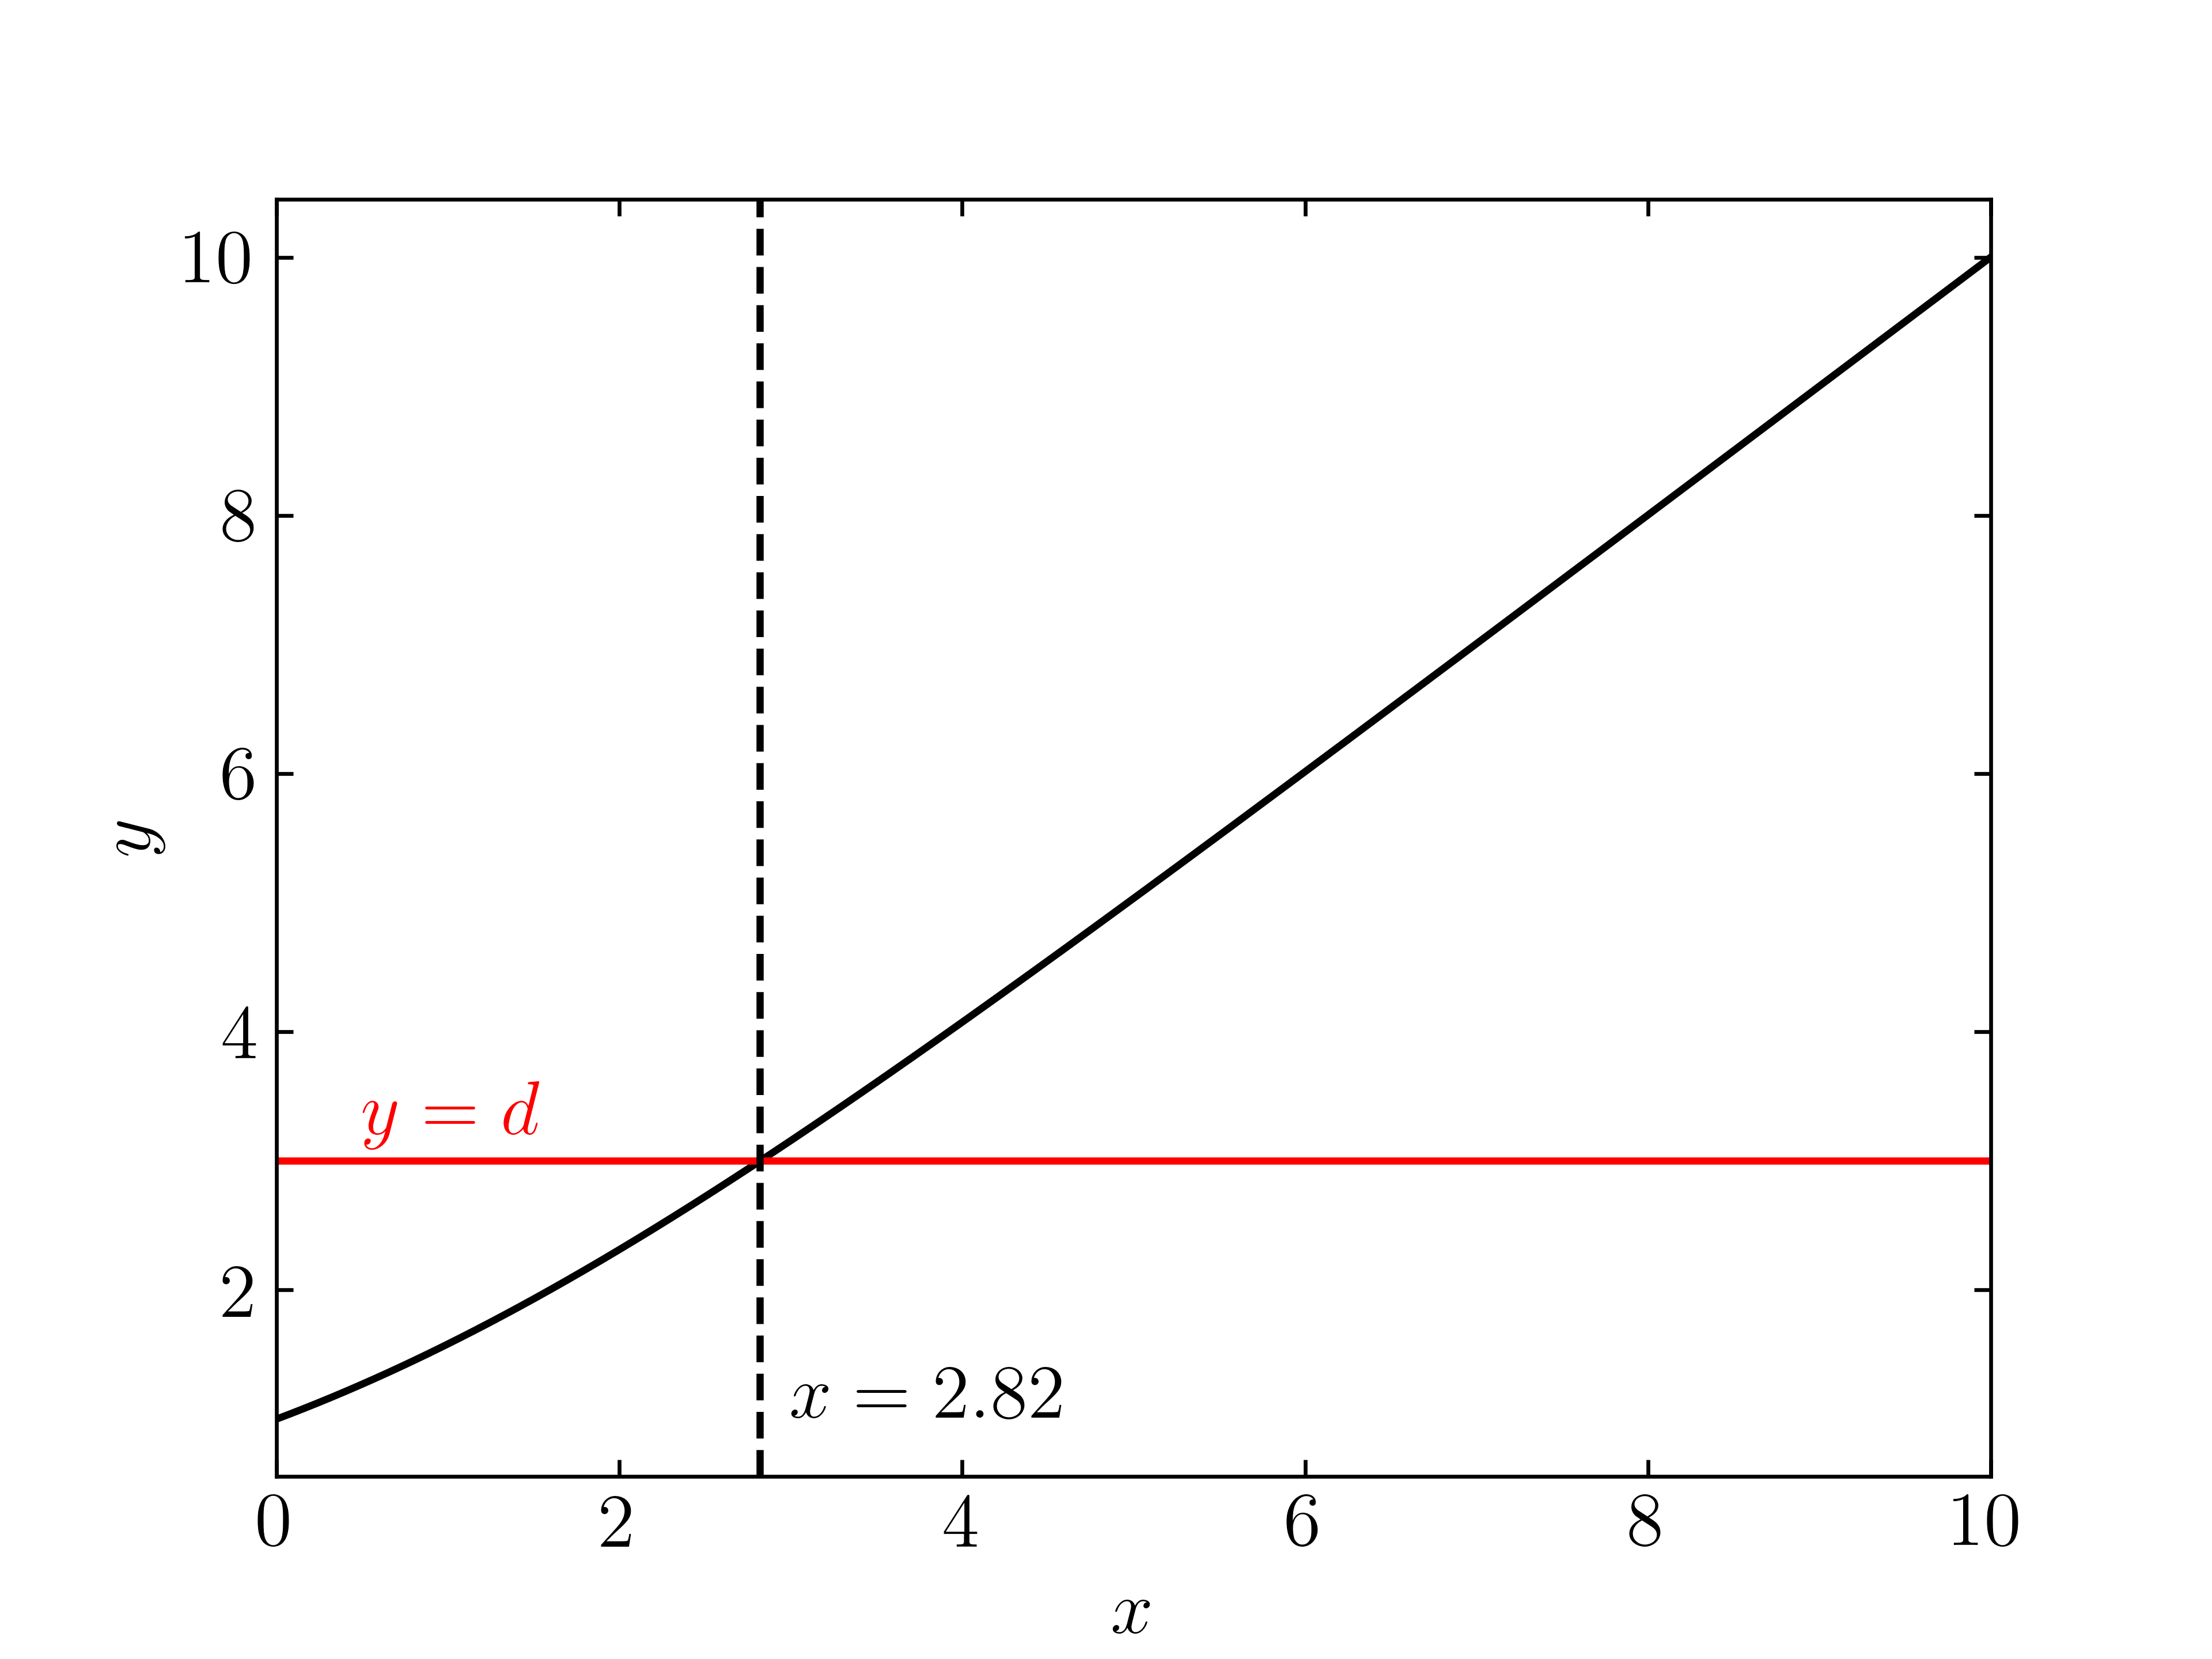
\includegraphics[width=0.8\textwidth]{p4.png} 
\end{center}
From the graph above, the root is at $x\approx 2.82$. Thus, the peak frequency
is
\begin{equation}
    f_p=\frac{\omega_p}{2\pi}=\frac{2.84}{2\pi}\frac{k_BT}{\hbar}. 
\end{equation}
For the average human body temperature, $T_\t{human}=310$\,\si{K}, leading to
$f_p\approx 18$\,\si{Hz}. For the average solar surface temperature
$T_\t{sun}=5772$\,\si{K}, the peak frequency is $f_p\approx 340$\,\si{THz}. This
is very close to the visible range from $\sim 400-790$\,\si{THz}, which makes
sense because the human eyes should be adapted to recognize the only prominent 
source of radiation in the solar system, which is the Sun.
\end{solution}

(f) Derive the relation between the pressure $P(T)$ (using $\ZZ$) and the energy
$E(T)$, verifying the characteristic result $P=(1/d)E/V$.

\textit{Hint}: (i) Note the very close relation of this problem to that of
finite temperature excitations above an atomic condensate. (ii) A
$d$-dimensional photon has $d-1$ polarizations (that you can take to be
degenerate) tranverse to the propagation wavevector $\vb{k}$. (iii) After
scaling out $T$ the integral can be reduced to a pure number that you can
compute via e.g., Mathematica. (iv) Refer to Hints in 3(d).
\begin{solution}
    First, we calculate the free energy
\begin{align}
    \FF&=-k_BT\ln\ZZ \notag\\
       &=2k_BT\sum_{\vb{k}}\ln\qty(1-e^{-\beta\hbar\omega})\notag\\
       &=2k_BT\frac{VS_d}{(2\pi)^d}\int_0^\infty dk
       k^{d-1}\ln\qty(1-e^{-\beta\hbar\omega})\notag\\
       &=Vk_BT\frac{2S_d}{(2\pi c)^d}\int_0^\infty
       d\omega\omega^{d-1}\ln\qty(1-e^{-\beta\hbar\omega})\notag\\
       &=-V\frac{2S_d\hbar}{d(2\pi \hbar c)^d}\int_0^\infty
       d\omega\frac{(\hbar\omega)^d}{e^{\beta\hbar\omega}-1}.
\end{align}
Then, the pressure is
\begin{equation}
    P=-\frac{\FF}{V}=\frac{2S_d}{(2\pi c)^d\hbar^{d-1}}\int_0^\infty
    d\omega\frac{(\hbar\omega)^d}{e^{\beta\omega}-1}. 
\end{equation}
Comparing this with \eqref{p4d:E}, we can write
\begin{equation}
    P=\frac1d\frac{E}{V}. 
\end{equation}
\end{solution}
\end{problem}
\newpage
%%%%%%%%%%%%%%%%%%%%%%%%%%%%%%%%%%%%%%%%%%%%%%%%%%%%%%%%%%%%%%%%%%%%%%%%%%%%%%%
%%%%%%%%%%%%%%%%%%%%%%%%%%%%%%%%%%%%%%%%%%%%%%%%%%%%%%%%%%%%%%%%%%%%%%%%%%%%%%%
\begin{problem}{5}[Phonons in a Debye solid]
As discussed in the lecture, there are only few more differences between
acoustic phonons and black-body phonons. These are (1) while acoustic phonon
dispersion $\omega_k$ is linear in $k$ near $k=0$, just like that of a photon,
with speed of light replaced by speed of sound, more generally phonon dispersion
is given by some nonlinear function $\omega_k$. (It is also typically quite
anisotropic, depending on $\vb{k}$ not just its magnitude $k$, but this we will
neglect). (2) Because phonons are normal modes of vibrations of discrete
periodic array of $N$ atoms, there only $N$ normal modes $\vb{k}$ and thus there
is a maximum value of $\vb{k}$ defining the Brillouin Zone of $N$ wavevectors
$\vb{k}$ values. (3) There are $d$ normal phonon modes per $\vb{k}$ rather than
$d-1$ of transverse photons. Since phonons are non-conserved excitations, they
are also characterized by a $\mu=0$.

As discussed in the lectures, we approximate true acoustic phonons with a `toy'
model of Debye phonons, taking $\omega_k$ to be linear in $k$ throughout, i.e.,
$v\hbar k$, for $k\leq k_\t{Debye}$, where the limiting $k_\t{Debye}$ is
determined by the constraint that there are a total of $N$ normal modes (per
polarization) in the crystal. Thus, the main crucial difference from the photons
is that there is a limiting upper $k_\t{Debye}$ and equivalently upper Debye
frequency, $\omega_\t{Debye}=vk_\t{Debye}$.

Armed with these facts, we will now fill in some of the details of the results
quoted in the lecture.

(a) Starting with the grand-canonical partition function, derive the integral
forms (over $\omega$) of the total energy $E(T)$ and the corresponding heat
capacity $C_v(T)$ in a $d$-dimensional isotropic Debye solid.
\begin{solution}
By definition, the grand-canonical partition function is
\begin{align}
    \ZZ&=\sum_\qty{n_{\vb{k},\alpha}}\exp\qty[-\beta E_\qty{n_{\vb{k},\alpha}}],
\end{align}
where
$E_\qty{n_{\vb{k},\alpha}}=\sum_{\vb{k},\alpha}\hbar\omega_{k,\alpha}n_{\vb{k},\alpha}$. Then, it follows that
\begin{align}
    \ZZ
    &=\sum_\qty{n_{\vb{k},\alpha}}\prod_{\vb{k}\in\t{BZ},\alpha}
    \exp\qty(-\beta n_{\vb{k},\alpha}\hbar\omega_{k,\alpha})\notag\\
    &=\prod_{\vb{k}\in\t{BZ},\alpha}\sum_{n_{\vb{k},\alpha}=0}^\infty
    \exp\qty(-\beta\hbar\omega_{k,\alpha})^{n_{\vb{k},\alpha}}\notag\\
    &=\prod_{\vb{k}\in\t{BZ},\alpha}\frac{1}{1-e^{-\beta\hbar\omega_{k,\alpha}}},
\end{align}
where BZ is the Brillouin Zone for each normal mode $\alpha$. Now, by 
definition, the energy is
\begin{align}
    E
    &=-\frac{\partial(\ln\ZZ)}{\partial\beta}\notag\\
    &=\sum_{\vb{k}\in\t{BZ},\alpha}\frac{\partial}{\partial\beta}\ln\qty(1-e^{-\beta\hbar\omega_{k,\alpha}})\notag\\
    &=\sum_{\vb{k}\in\t{BZ},\alpha}\frac{\hbar\omega_{k,\alpha}}{e^{\beta\hbar\omega_{k,\alpha}}-1}.\notag\\
    &=\int
    d\omega\sum_{\vb{k}\in\t{BZ},\alpha}\delta(\omega-\omega_{k,\alpha})\frac{\hbar\omega}{e^{\beta\hbar\omega}-1}\notag\\
    &=\int d\omega g(\omega)\frac{\hbar\omega}{e^{\beta\hbar\omega}-1},
\end{align}
where the density of states is
\begin{align}
    g(\omega)
    &=\sum_{\vb{k}\in\t{BZ},\alpha}\delta(\omega-\omega_{k,\alpha}) \notag\\
    &=\sum_{\vb{k}\in\t{BZ}}\delta(\omega-c_Lk)+(d-1)\sum_{\vb{k}\in\t{BZ}}\delta(\omega-c_Tk)\notag\\
    &=V\int_\t{BZ}\frac{d^dk}{(2\pi)^d}\qty[\delta(\omega-c_Lk)+(d-1)\delta(\omega-c_Tk)]\notag\\
    &=V\frac{S_d}{(2\pi)^d}\int_0^{k_D}dkk^{d-1}\qty[\frac1{c_L}\delta(k-\frac{\omega}{c_L})+\frac{d-1}{c_T}\delta(k-\frac{\omega}{c_T})]\notag\\
    &=\frac{V}{\Gamma(d/2)2^{d-1}\pi^{d/2}}\qty(\frac1{c_L^d}+\frac{d-1}{c_T^d})\omega^{d-1},
\end{align}
for $\omega<\omega_D$ and zero otherwise. $c_T,c_L$ are the transverse
and longitudinal acoustic speed. The constraint for the number of modes is
\begin{equation}
    dN=\int g(\omega)d\omega
    =\frac{V}{\Gamma(d/2)2^{d-1}\pi^{d/2}}\qty(\frac1{c_L^d}+\frac{d-1}{c_T^d})\frac{\omega_D^d}{d}.
\end{equation}
Thus, the Debye frequency is determined by
\begin{equation}
    \omega_D^d=d^2\Gamma(d/2)2^{d-1}\pi^{d/2}\frac{N}V\qty(\frac1{c_L^d}+\frac{d-1}{c_T^d})^{-1}.
\end{equation}
This gives a simplified form for the density of states
\begin{equation}
    g(\omega)=d^2N\frac{\omega^{d-1}}{\omega_D^d}.
\end{equation}
Plugging this in, we get the energy
\begin{equation}
    E=\frac{d^2N}{\hbar^{d-1}\omega_D^d}\int_0^{\omega_D}d\omega\frac{(\hbar\omega)^d}{e^{\beta\hbar\omega}-1}.
\end{equation}
Then, we can also calculate
\begin{equation}
    C_V=\frac{\partial E}{\partial T}
    =\frac{d^2Nk_B\beta^2}{\hbar^{d-1}\omega_D^d}\int_0^{\omega_D}d\omega\frac{(\hbar\omega)^{d+1}e^{\beta\hbar\omega}}{(e^{\beta\hbar\omega}-1)^2}.
\end{equation}
\end{solution}

(b) Based on your analytic integral expression for $C_v(T)$, argue that (i) for
$k_BT\ll \hbar\omega_D$, the result reduces to that of the black-body heat
capacity, and in contrast (ii) for $k_BT\gg \hbar\omega_D$, heat capacity
crosses over (plateaus to) the equipartition value, as expected. What is the
number of degrees of freedom that this gives in $d$ dimensions?
\begin{solution}
Letting $x=\beta\hbar\omega$, the expression for $C_v$ becomes
\begin{align}\label{p5b:Cv}
    C_v=\frac{d^2Nk_B}{x_D^d}\int_0^{x_D}dx\frac{x^{d+1}e^x}{(e^x-1)^2},
\end{align}
where $x_D=\beta\hbar\omega_D$. For $x_D\to\infty$, the integral converges to
some finite value. Thus, $C_v\sim x_D^{-d}\sim T^d$, similar to the black-body
result attained in the previous problem. On the other hand, if $x_D$ is small,
then the integrand can be expanded to lowest order in $x$,
\begin{align}
    C_v(x_D\ll 1)\approx\frac{d^2Nk_B}{x_D^d}\int_0^{x_D}dx x^{d-1}
    =dNk_B,
\end{align}
resulting in equipartition in $dN$ degrees of freedom.
\end{solution}

(c) Sketch $C_v(T)$ as a function of $T$ for a fixed value of Debye frequency
$\omega_D$, paying attention to the behavior of the expression for $T$ relative
to $\hbar\omega_D/k_B$. Check your sketch with Mathematica.
\begin{solution}
Below, we plot \eqref{p5b:Cv} in terms of $x$.
\begin{center}
    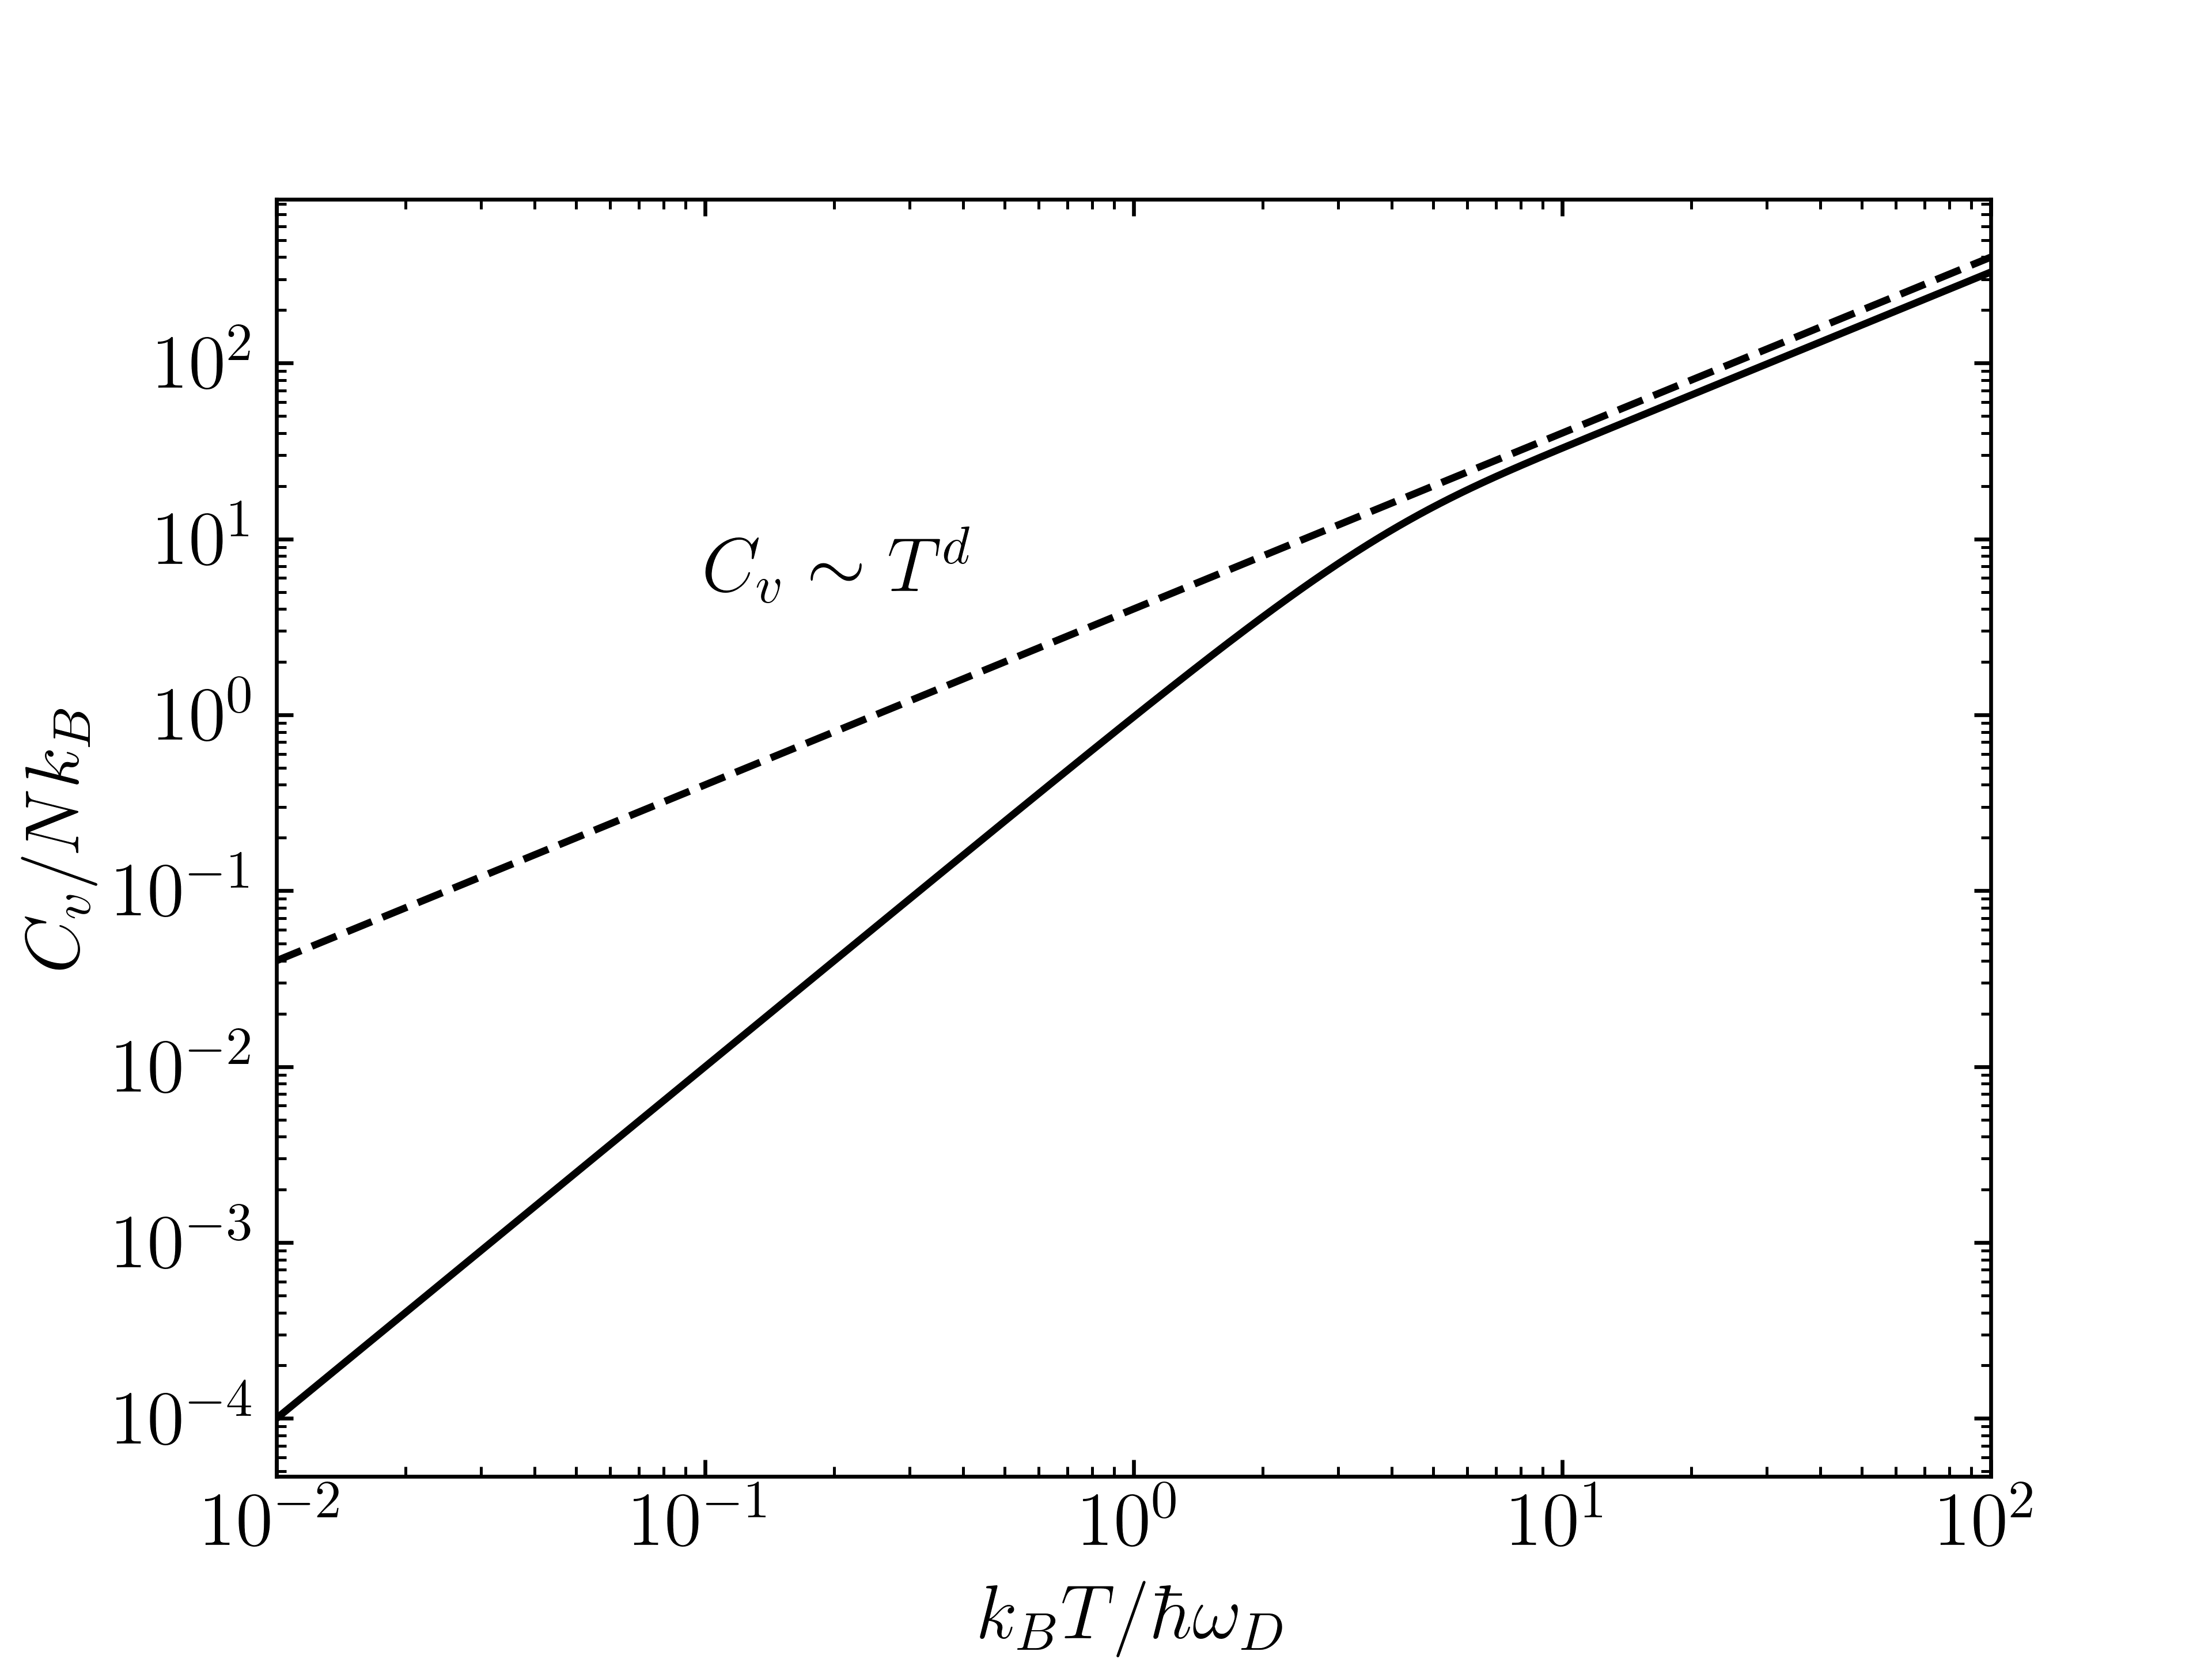
\includegraphics[width=0.8\textwidth]{p5.png} 
\end{center}
The transition temperature is a bit higher than $x=1$, albeit on the same order
of magnitude. At low temperature, the system freezes out, while at high
temperature, $C_v$ approaches the black-body behaviors.
\end{solution}
\end{problem}
\newpage
%%%%%%%%%%%%%%%%%%%%%%%%%%%%%%%%%%%%%%%%%%%%%%%%%%%%%%%%%%%%%%%%%%%%%%%%%%%%%%%
%%%%%%%%%%%%%%%%%%%%%%%%%%%%%%%%%%%%%%%%%%%%%%%%%%%%%%%%%%%%%%%%%%%%%%%%%%%%%%%
\begin{problem}{6}[Fermi gas thermodynamics: electrons in a metal]
In lectures we introduced noninteracting (ideal) Fermi gas in a box (with
periodic boundary conditions) and presented many results, some without
derivations. Here I will ask you to derive some of the details.

The theory describes thermodynamics of any gas (noninteracting) of $N$ fermionic
particles. The most important applications of this theory is to that of the
electrons confined inside of a piece of metal. It also describes a neutron star
composed of neutrons, as well as trapped fermionic atomic gases, such as e.g.,
$\t{K}^{40}$ as first cooled to degeneracy by Professor Debbie Jin in her
seminal work dating back to 1999.

(a) Details of the Fermi distribution function

Starting from the fermionic grand-partition function $\ZZ$, we wrote don the
expression for the expectation value for the occupation of the $\alpha$
single-particle state, namely
$\expval{n_\alpha}_F=1/\qty[e^{(\epsilon_\alpha-\mu)/k_BT}+1]$, the so-called
Fermi-Dirac distribution.
\begin{enumerate}[label=(\roman*)]
    \item Derive $n_F(\epsilon_k)$ from the fermionic grand-partition function $\ZZ$
for spinless fermions. How does it trivially extend for spin-1/2 electrons in
zero magnetic field?
\item Plot $n_F(\epsilon_k)$ and its derivative
$\partial_{\epsilon_k}n_F(\epsilon_k)$ for fixed positive chemical potential
$\mu>0$ as a function of $\epsilon_k$ for a series of $k_BT/\mu$ values,
covering high (Boltzmann gas) and low (degenerate gas) temperature limits.
\item Combine above graphical analysis with analytical examination of
    $n_F(\epsilon_k)$ in $T\to0$ limit to show that at $T=0$, it becomes a step
    function $\theta(\epsilon_k-\mu)$ at $\mu=\epsilon_F$ and $\partial_\epsilon
    n_F(\epsilon)=A\delta(\epsilon-\epsilon_F)$ a $\delta$-function, where
    $\epsilon_F=\mu(T=0)$. What is the amplitude of $A$ of the
    $\delta$-function?
\end{enumerate}
\begin{solution}
(i) The energy eigenvalues for spinless fermions are
\begin{equation}
    \epsilon_k=\frac{\hbar^2k^2}{2m}. 
\end{equation}
Thus, the FD distribution is
\begin{equation}\label{p6ai:nf}
    n_F=\frac1{e^{\beta(\epsilon_k-\mu)}+1}
    =\frac1{e^{\beta(\hbar^2k^2/2m-\mu)}+1}.
\end{equation}
For spin-1/2 electrons, the energy eigenvalues are
\begin{equation}
    \epsilon_k=\frac{\hbar^2k^2}{2m}+\sigma\mu_BB, 
\end{equation}
for $\sigma\in\qty{1,-1}$. However, in zero magnetic field, they are the same as
the spinless case. Thus, the FD distribution for them is also the same as
\eqref{p6ai:nf}.

(ii) The derivative of \eqref{p6ai:nf} is
\begin{equation}
    \frac{\partial
    n_F}{\partial\epsilon_k}=-\beta\frac{e^{\beta(\epsilon_k-\mu)}}{(e^{\beta(\epsilon-\mu)}+1)^2}. 
\end{equation}
Below, we plot $n_F$ (upper pannel) and $\partial n_F/\partial x$ (lower panel) where $x=\beta\epsilon_k$.
\begin{center}
    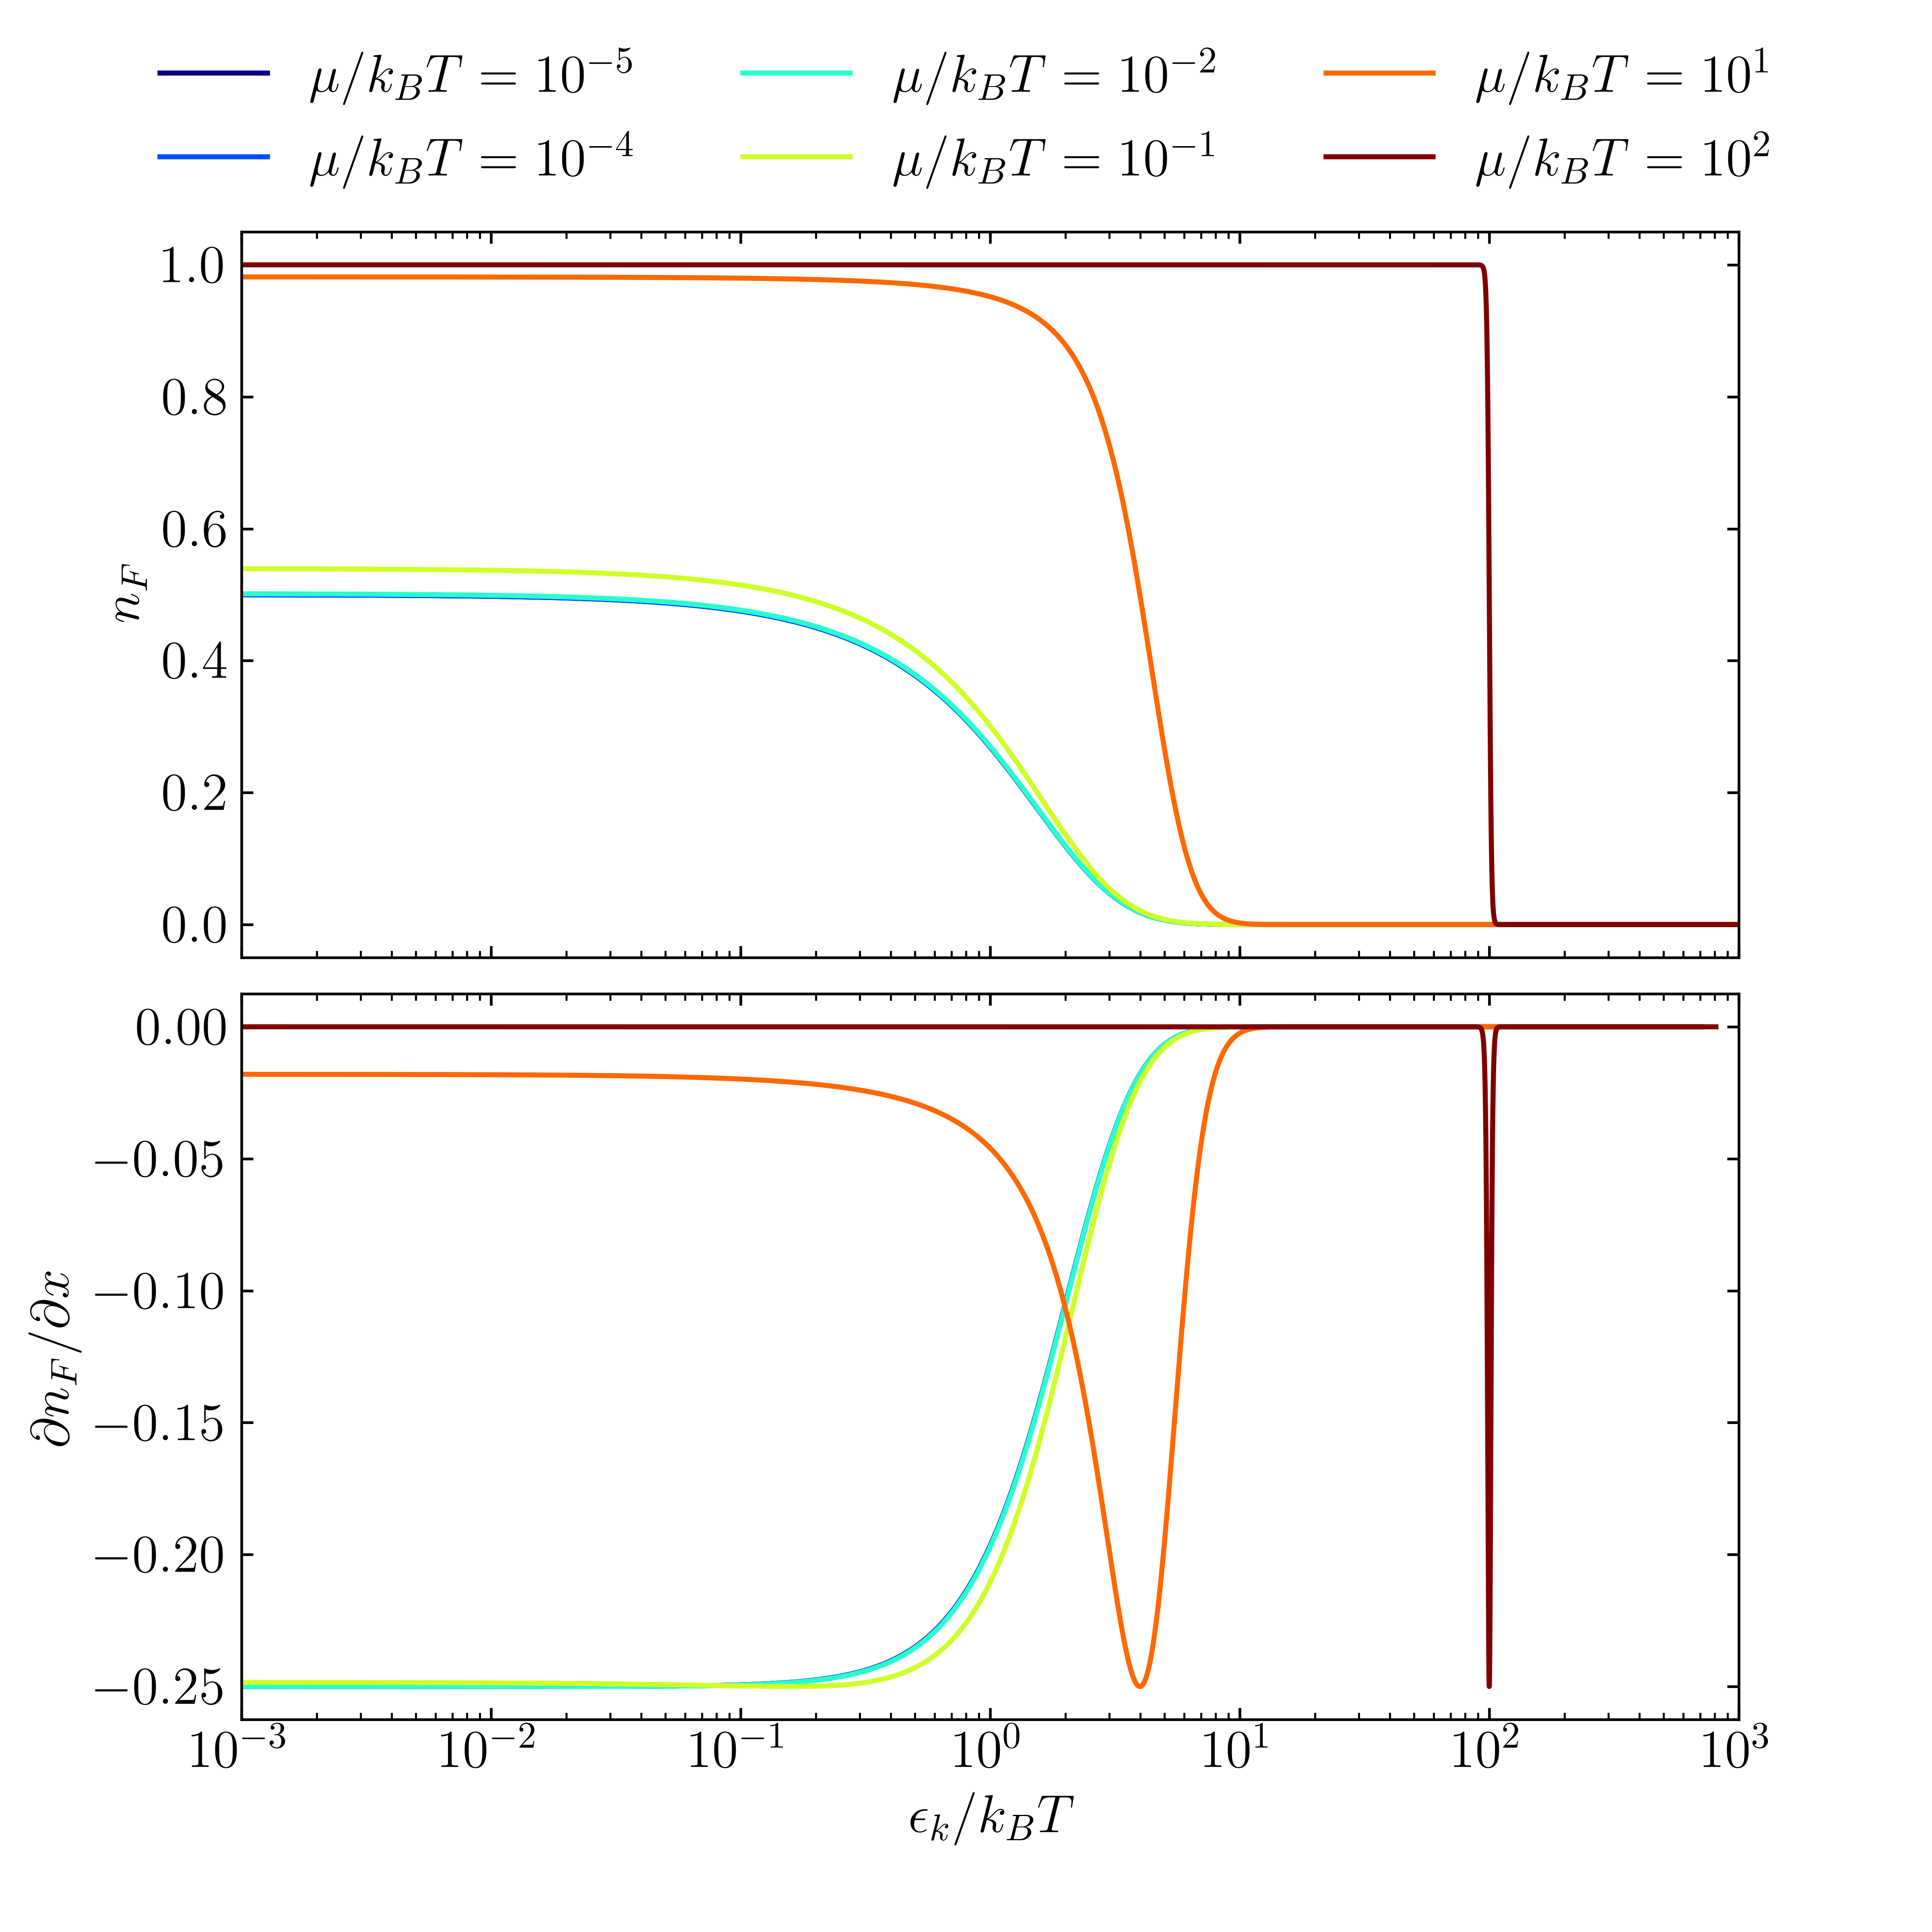
\includegraphics[width=0.8\textwidth]{p6.png} 
\end{center}

(iii) Indeed, $n_F$ becomes a step function $\theta(\epsilon_k-\mu)$, while
$n_F'$ becomes a delta function as $T\to0$. Also, by inspection, at
$\mu=\epsilon_k$, we can evaluate
\begin{equation}
    \frac1\beta\frac{\partial
    n_F}{\partial\epsilon_k}=-\frac{e^{\beta(\epsilon-\mu)}}{(e^{\beta(\epsilon-\mu)}+1)^2}=-\frac14. 
\end{equation}
Thus, the amplitude of the delta function is $-1/4$. As seen in the second
panel, all curves reach minimum at $-0.25$.
\end{solution}

(b) Zero-temperature Fermi gas analysis
\begin{enumerate}[label=(\roman*)]
    \item Let's reexamine the number $N$ equation for $T=0$. Use the above
        derived $T=0$ form of the Fermi function to compute the right hand side
        of the $N$ equation, and thereby derive the relation between the Fermi
        energy $\epsilon_F(n)$ (upper limit of the energy $\epsilon$ integral)
        and the density $n$ in $d$ dimensions.

        \textit{Hint}: (i) Notice that in this $T=0$ limit, the step-function of
        amplitude 1 just corresponds to filling al the lowest energy states
        $\vb{k}$ at single-particle energies $\epsilon_{\vb{k}}$ one by one with
        $N$ fermions (one per $\vb{k}$, since we ignore electron spin -- think
        of it as being polarized by a strong external $B$ field and thus only
        one lowest spin state matters), corresponding to the highest Fermi
        energy, $\epsilon_F$. (ii) In this imit the integral is trivial exercise
        in $d$ dimensional calculus, that we already extensively discussed (do
        the integral over angular variables getting $S_d$, followed by a simple
        radial $k$ integral up to $k_F$). (iii) Check your answer based on
        dimensional analysis, recalling our discussion of the degeneracy energy
        $k_BT_\ast$ in the lecture.

    \item Calculate the \textit{total} many-body energy
        $E(n)=\sum_{\vb{k}}\epsilon_{\vb{k}}n_F(\epsilon_{\vb{k}})$ as a
        function of the fermion density in $d$ dimensions. Do it in the
        thermodynamic limit where the sum over $\vb{k}$ can be replaced by
        appropriate $\vb{k}$ integral, as in the number equation problem, above.
        Check that your answer satisfies the dimensional analysis, and noting
        that $E(n)$ can be written in terms of $n$ and $\epsilon_F(n)$ derived
        above.

    \item What is the equivalent Fermi temperature, $T_F=E_F/k_B$ for electrons
        in a metal like Sodium, Na? At this energy, what is the velocity of the
        electron at this kinetic energy? Be amazed at this Pauli principle
        enforced result, given that the electrons are at zero temperature.

    \textit{Hint}:  Atoms in a crystal are typically an Angstrom apart (that's
    because atoms are about an Angstrom in size as you know from study of the
    hydrogen atom), with each donating an electron (in Alkali atoms of the first
    coumn of the periodic table), thereby setting the electron spacing and their
    corresponding number density. The associated energy is a familiar energy
    that you all encountered corresponding to an eectron's kinetic eneryg
    associated with deBroglie wavelength of an Angstrom, thereby not really
    requiring any further calculations (but you are welcome to put the numbers
    in to verify the answer).
\end{enumerate}
\begin{solution}
(i) By definition, at $T=0$, $\mu=\epsilon_F$ and
\begin{align}
    N&=\sum_{\vb{k}}\theta(\epsilon_k-\epsilon_F) \notag\\
     &=\frac{V}{(2\pi)^d}S_d\int_0^{k_F} dk
     k^{d-1}\notag\\
     &=\frac{V}{\Gamma(d/2)(4\pi)^{d/2}}\qty(\frac{2m}{\hbar^2})^{d/2}
     \int_0^{\epsilon_F}d\epsilon \epsilon^{d/2-1}\notag\\
     &=\frac{2}{d}\frac{V}{\Gamma(d/2)}\frac1{\lambda^d}\qty(\frac{\epsilon_F}{k_BT})^{d/2}.
\end{align}
We can then invert to write
\begin{equation}\label{p6b:eps}
    \epsilon_F(n)=k_BT\qty[\Gamma(d/2+1)(n\lambda^d)]^{2/d}. 
\end{equation}

(ii) Similarly, we can also calculate
\begin{align}
    E(n)&=\frac{V}{(2\pi)^d}\int
    d^dk\epsilon_k\theta(\epsilon_k-\epsilon_F)\notag\\
        &=\frac{V}{(2\pi)^d}\frac{\pi^{d/2}}{\Gamma(d/2)}\qty(\frac{2m}{\hbar^2})^{d/2}\int_0^{\epsilon_F}d\epsilon
        \epsilon^{d/2}\notag\\
        &=\frac{V}{(d/2+1)\Gamma(d/2)}\frac1{\lambda^d}\qty(\frac{\epsilon_F}{k_BT})^{d/2}\epsilon_F\notag\\
        &=\frac{d/2}{d/2+1}N\epsilon_F\notag\\
        &=\frac{d}{d+2}Nk_BT\qty[\Gamma(d/2+1)(n\lambda^d)]^{2/d}.
\end{align}
The dimensions make sense.

(iii) From Google, the Fermi energy of sodium is 3.24\,\si{eV}. Thus, the
equivalent Fermi temperature is $T_F\approx3.76\times10^4$\,\si{K}, and the
velocity of electrons at this temperature is
$v=\sqrt{2T/m_e}\approx1.1\times10^6$\,\si{m/s}.
\end{solution}

(c) Nonzero-temperature Fermi gas analysis

For electron as we discussed at high temperature $T\gg T_\ast$, the gas is
nondegenerate and its phenomenology is that of the Boltzmann gas, with e.g.,
$\mu(T)\sim -T\ln T$, independent of whether the particles are fermions or
bosons. However, in contrast to bosons, for fermions the chemical potential
crosses zero and becomes positive in the degenerate, low-temperature regime
$T<T_\ast$, at $T=0$ saturating at a value that is named Fermi energy,
$\epsilon_F=\hbar^2k_F^2/2m$, where $\hbar k_F$ is the so-called Fermi momentum
defined by above expression, corresponding to the Fermi wavevector $k_F$,
denoting the highest momentum state occupied at $T=0$. This behavior is valid
for Fermi gas in any dimension, but is particularly simple to work out in two
dimensions (2d).

\begin{enumerate}[label=(\roman*)]
    \item Write down the number equation $N$ in 2d and carry out the momentum
        integral exactly, thereby finding $\mu(T,n)$.

        \textit{Hint}: It is convenient to change variables to
        $x=\beta(\epsilon_k-\mu)$ and then rewrite the resulting integrand in
        terms of $e^{-x}$, which gives a nice Jacobian for a straightforward
        exact integration.

    \item Analyze the resulting analytical expression $\mu(T,n)$ for high- and
        low-temperatures limits with respect to $T_\ast$ (i.e., the Fermi
        temperature $T_F=\epsilon_F/k_B$), recovering the expected Boltzmann gas
        behavior and asymptotic temperature independent Fermi energy
        $\epsilon_F(n)$ value as a function of the density, found above.

    \item Plot this 2d result for $\mu(T,n)$ for high and low temperatures as a
        function of $T$.

    \item At low temperature $T\ll T_F$ compute $E(T,n)$ nd the corresponding
        heat capacity $C_V(T,n)$, noting the expected failure of the
        equipartition.

    \textit{Hint}: Do this only as the lowest order in $T/T_F$ correction to the
    zero-temperature total energy $E(n)$ computed above.
\end{enumerate}
\begin{solution}
(i) By definition, the exact number equation is
\begin{align}
    N
    &=\sum_{\vb{k}}\frac1{e^{\beta(\epsilon_k-\mu)}}\notag\\
    &=\frac{L^2}{(2\pi)^2}2\pi\int_0^\infty dk
    \frac{k}{e^{\beta(\epsilon-\mu)}+1}\\
    &=\frac{L^2}{2\pi}\frac{m}{\hbar^2}\int_0^\infty\frac{d\epsilon}{e^{\beta(\epsilon-\mu)}+1}\notag\\
    &=\qty(\frac{L}{\lambda})^2\int_{-\mu\beta}^\infty \frac{dx}{e^x+1}\notag\\
    &=\qty(\frac{L}{\lambda})^2\sum_{n=1}^\infty(-1)^{n-1}\int_{-\mu\beta}^\infty
    dxe^{-nx}\notag\\
    &=\qty(\frac{L}{\lambda})^2\sum_{n=1}^\infty
    (-1)^{n-1}\frac{e^{n\mu\beta}}{n}\notag\\
    &=\qty(\frac{L}{\lambda})^2\ln(1+e^{\mu\beta}).
\end{align}
Inverting this yields
\begin{equation}
    \mu(T,n)=k_BT\ln\qty(e^{n\lambda^2}-1)
    =k_BT\ln\qty(e^{\epsilon_F/k_BT}-1), 
\end{equation}
where $n=N/A$ and we have used previous result \eqref{p6b:eps}. Letting
$\epsilon_F=k_BT_\ast$, the chemical potential becomes
\begin{equation}
    \frac{\mu}{k_BT_\ast}=\frac{T}{T_\ast}\ln\qty(e^{T_\ast/T}-1). 
\end{equation}

(ii) For large temperature $T\gg T_\ast$, $e^{T_\ast/T}-1\approx T_\ast/T$ and
we recover the classical Boltzmann gas result
\begin{equation}
    \frac{\mu}{k_BT_\ast}\approx -\frac{T}{T_\ast}\ln\qty(\frac{T}{T_\ast}). 
\end{equation}
In the opposite end, at low temperature $T\ll T_\ast$, the exponential term
dominates unity and the chemical potential $\mu/k_BT_\ast\approx
(T/T_\ast)\ln(e^{T_\ast/T})=1$, which is consistent with $\mu(T=0)=\epsilon_F$.

(iii) Below, the plotted chemical potential saturates as expected.
\begin{center}
    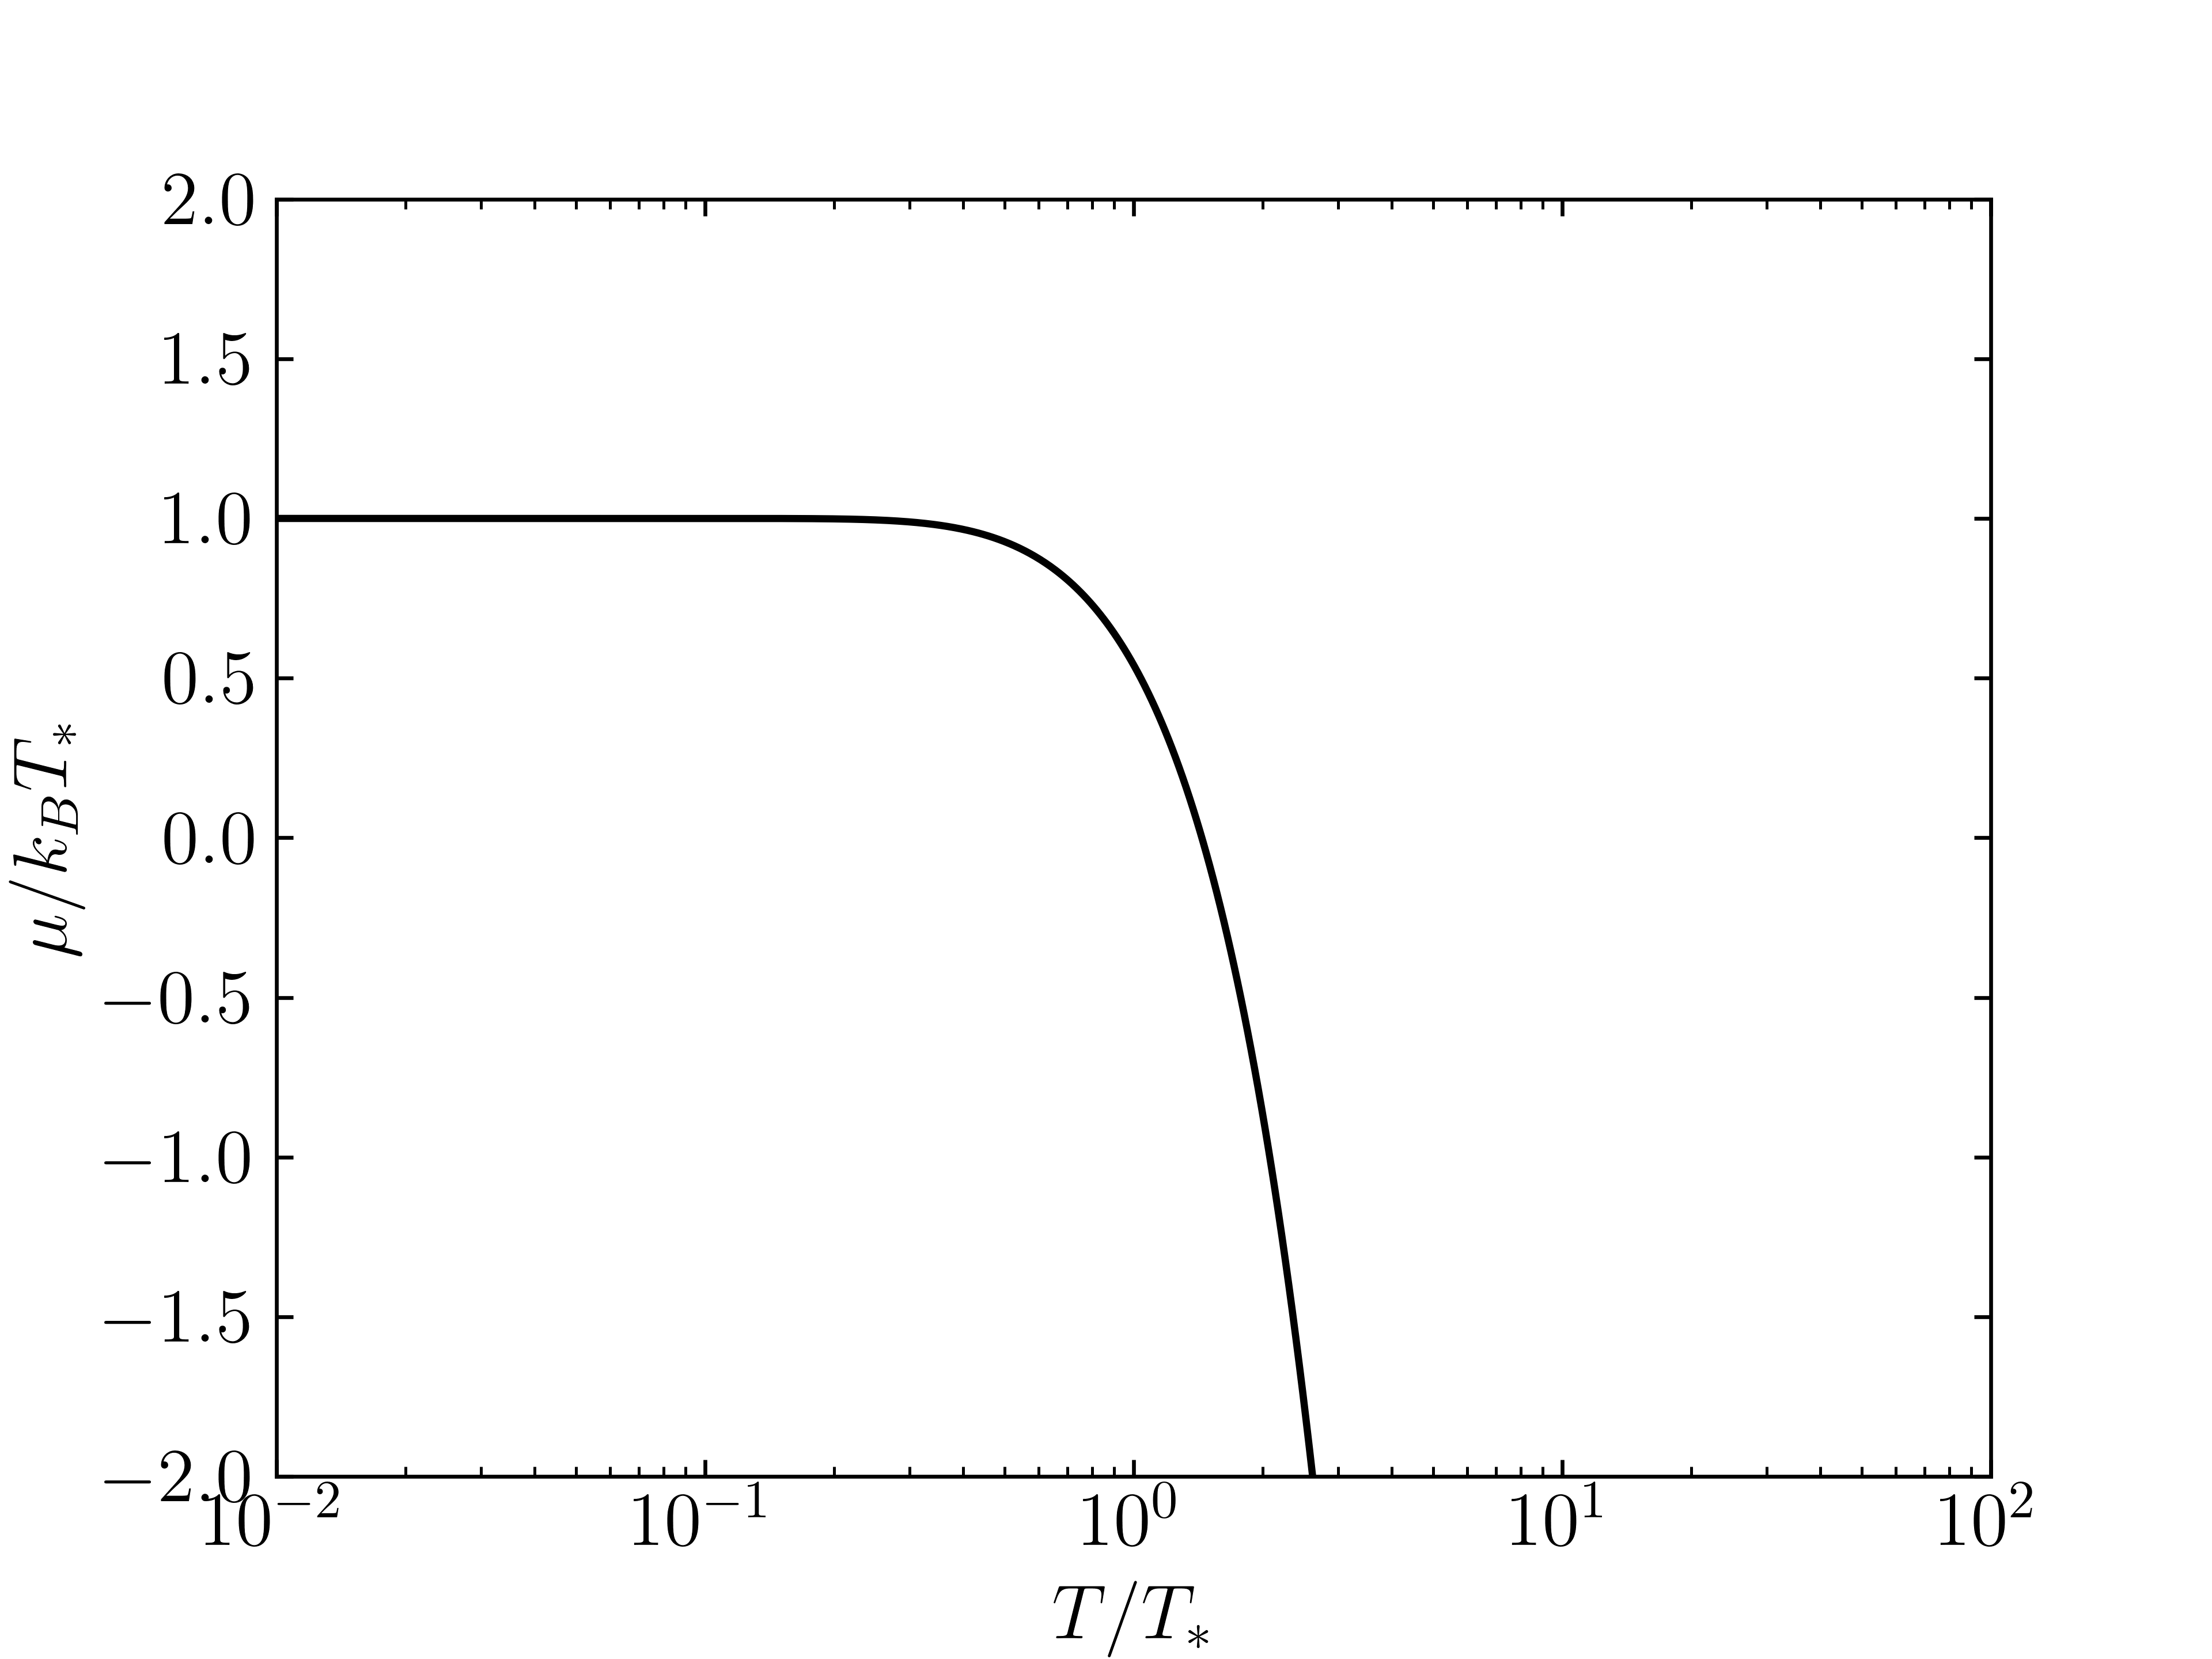
\includegraphics[width=0.8\textwidth]{p6c.png} 
\end{center}

(iv) At $T\ll T_\ast$, $\mu=\epsilon_F$ and we can calculate
\begin{align}
    E(n)
    &=\sum_{\vb{k}}\frac{\epsilon_k}{e^{\beta(\epsilon_k-\epsilon_F)}+1}\notag\\
    &\approx\frac{L^2m}{2\pi\hbar^2}\int_0^\infty \epsilon
    e^{\beta(\epsilon-\epsilon_F)}d\epsilon\notag\\
    &=\qty(\frac{L}{\lambda})^2k_BTe^{-\beta\epsilon_F}\notag\\
    &\approx \qty(\frac{L}{\lambda})^2k_BT,
\end{align}
to the lowest order. It then follows that $C_v=(L/\lambda)^2k_B$, which doesn't
satisfy equipartition.
\end{solution}
\end{problem}
\newpage
%%%%%%%%%%%%%%%%%%%%%%%%%%%%%%%%%%%%%%%%%%%%%%%%%%%%%%%%%%%%%%%%%%%%%%%%%%%%%%%
\end{document}
